\documentstyle[11pt,epsfig]{article}
\pagestyle{myheadings}

% -----------------------------------------------------------------------------
% ? Document identification
\newcommand{\stardoccategory}  {Starlink User Note}
\newcommand{\stardocinitials}  {SUN}
\newcommand{\stardocsource}    {sun\stardocumber}
\newcommand{\stardocnumber}    {223.0}
\newcommand{\stardocauthors}   {D.S. Berry \& T.M. Gledhill }
\newcommand{\stardocdate}      {16 April 1998}
\newcommand{\stardoctitle}     {POLPACK}
\newcommand{\stardoconeline}   {A Dual-beam imaging polarimetry reduction package}
\newcommand{\stardocversion}   {Version 1.0}
\newcommand{\stardocmanual}    {Users' Manual}
% ? End of document identification
% -----------------------------------------------------------------------------

\newcommand{\stardocname}{\stardocinitials /\stardocnumber}
\markright{\stardocname}
\setlength{\textwidth}{160mm}
\setlength{\textheight}{230mm}
\setlength{\topmargin}{-2mm}
\setlength{\oddsidemargin}{0mm}
\setlength{\evensidemargin}{0mm}
\setlength{\parindent}{0mm}
\setlength{\parskip}{\medskipamount}
\setlength{\unitlength}{1mm}

% -----------------------------------------------------------------------------
%  Hypertext definitions.
%  ======================
%  These are used by the LaTeX2HTML translator in conjunction with star2html.

%  Comment.sty: version 2.0, 19 June 1992
%  Selectively in/exclude pieces of text.
%
%  Author
%    Victor Eijkhout                                      <eijkhout@cs.utk.edu>
%    Department of Computer Science
%    University Tennessee at Knoxville
%    104 Ayres Hall
%    Knoxville, TN 37996
%    USA

%  Do not remove the %\begin{rawtex} and %\end{rawtex} lines (used by
%  star2html to signify raw TeX that latex2html cannot process).
%\begin{rawtex}
\makeatletter
\def\makeinnocent#1{\catcode`#1=12 }
\def\csarg#1#2{\expandafter#1\csname#2\endcsname}

\def\ThrowAwayComment#1{\begingroup
    \def\CurrentComment{#1}%
    \let\do\makeinnocent \dospecials
    \makeinnocent\^^L% and whatever other special cases
    \endlinechar`\^^M \catcode`\^^M=12 \xComment}
{\catcode`\^^M=12 \endlinechar=-1 %
 \gdef\xComment#1^^M{\def\test{#1}
      \csarg\ifx{PlainEnd\CurrentComment Test}\test
          \let\html@next\endgroup
      \else \csarg\ifx{LaLaEnd\CurrentComment Test}\test
            \edef\html@next{\endgroup\noexpand\end{\CurrentComment}}
      \else \let\html@next\xComment
      \fi \fi \html@next}
}
\makeatother

\def\includecomment
 #1{\expandafter\def\csname#1\endcsname{}%
    \expandafter\def\csname end#1\endcsname{}}
\def\excludecomment
 #1{\expandafter\def\csname#1\endcsname{\ThrowAwayComment{#1}}%
    {\escapechar=-1\relax
     \csarg\xdef{PlainEnd#1Test}{\string\\end#1}%
     \csarg\xdef{LaLaEnd#1Test}{\string\\end\string\{#1\string\}}%
    }}

%  Define environments that ignore their contents.
\excludecomment{comment}
\excludecomment{rawhtml}
\excludecomment{htmlonly}
%\end{rawtex}

%  Hypertext commands etc. This is a condensed version of the html.sty
%  file supplied with LaTeX2HTML by: Nikos Drakos <nikos@cbl.leeds.ac.uk> &
%  Jelle van Zeijl <jvzeijl@isou17.estec.esa.nl>. The LaTeX2HTML documentation
%  should be consulted about all commands (and the environments defined above)
%  except \xref and \xlabel which are Starlink specific.

\newcommand{\htmladdnormallinkfoot}[2]{#1\footnote{#2}}
\newcommand{\htmladdnormallink}[2]{#1}
\newcommand{\htmladdimg}[1]{}
\newenvironment{latexonly}{}{}
\newcommand{\hyperref}[4]{#2\ref{#4}#3}
\newcommand{\htmlref}[2]{#1}
\newcommand{\htmlimage}[1]{}
\newcommand{\htmladdtonavigation}[1]{}

%  Starlink cross-references and labels.
\newcommand{\xref}[3]{#1}
\newcommand{\xlabel}[1]{}

%  LaTeX2HTML symbol.
\newcommand{\latextohtml}{{\bf LaTeX}{2}{\tt{HTML}}}

%  Define command to re-centre underscore for Latex and leave as normal
%  for HTML (severe problems with \_ in tabbing environments and \_\_
%  generally otherwise).
\newcommand{\latex}[1]{#1}
\newcommand{\setunderscore}{\renewcommand{\_}{{\tt\symbol{95}}}}
\latex{\setunderscore}

%  Redefine the \tableofcontents command. This procrastination is necessary
%  to stop the automatic creation of a second table of contents page
%  by latex2html.
\newcommand{\latexonlytoc}[0]{\tableofcontents}

% -----------------------------------------------------------------------------
%  Debugging.
%  =========
%  Remove % on the following to debug links in the HTML version using Latex.

% \newcommand{\hotlink}[2]{\fbox{\begin{tabular}[t]{@{}c@{}}#1\\\hline{\footnotesize #2}\end{tabular}}}
% \renewcommand{\htmladdnormallinkfoot}[2]{\hotlink{#1}{#2}}
% \renewcommand{\htmladdnormallink}[2]{\hotlink{#1}{#2}}
% \renewcommand{\hyperref}[4]{\hotlink{#1}{\S\ref{#4}}}
% \renewcommand{\htmlref}[2]{\hotlink{#1}{\S\ref{#2}}}
% \renewcommand{\xref}[3]{\hotlink{#1}{#2 -- #3}}
% -----------------------------------------------------------------------------
% ? Document specific \newcommand or \newenvironment commands.

% Environment for indenting and using a small font.
\newenvironment{myquote}{\begin{quote}\begin{small}}{\end{small}\end{quote}}

% In-line typed text, buttons and menu items.
\newcommand{\butt}[1]{{\small \bf \tt #1}}
\newcommand{\menu}[1]{{\small \bf \em #1}}
\newcommand{\wlab}[1]{{\small \bf #1}}
\newcommand{\text}[1]{{\small \tt #1}}

% Quick routine descriptions
\newcommand{\quickdes}[3]{
                         \parbox{1.1in}{\bf #1}
                         \parbox{4.4in}{\raggedright #2 \dotfill}
                         \parbox{0.6in}{\pageref{#3}}
                         \vspace*{0.2in}}

% Quotes for SST.
\newcommand{\qt}[1]{{\tt "}#1{\tt "}}
\newcommand{\qs}[1]{{\tt '}#1{\tt '}}
\begin{htmlonly}
   \renewcommand{\qt}[1]{ {\tt{"}}#1{\tt{"}} }
   \renewcommand{\qs}[1]{ {\tt{'}}#1{\tt{'}} }
\end{htmlonly}

% Routines with descriptions in the appendix.
\newcommand{\routine}[1]{{\sc #1}}
\newcommand{\xroutine}[1]{\htmlref{{\sc #1}}{#1}}

% Latex only sections, subsections etc. Surround these with a latexonly
% environment.
\newcommand{\latexonlysection}[1]{\section{#1}}
\newcommand{\latexonlysubsection}[1]{\subsection{#1}}
\newcommand{\latexonlysubsubsection}[1]{\subsubsection{#1}}
\begin{htmlonly}
   \newcommand{\latexonlysection}[1]{#1}
   \newcommand{\latexonlysubsection}[1]{#1}
   \newcommand{\latexonlysubsubsection}[1]{#1}
\end{htmlonly}

% degrees symbol
\newcommand{\dgs}{\hbox{$^\circ$}} 
\begin{htmlonly}
\renewcommand{\dgs}{{\rawhtml &deg;}} 
\end{htmlonly}

% ? End of document specific commands
% -----------------------------------------------------------------------------
%  Title Page.
%  ===========
\renewcommand{\thepage}{\roman{page}}
\begin{document}
\thispagestyle{empty}

%  Latex document header.
%  ======================
\begin{latexonly}
   CCLRC / {\sc Rutherford Appleton Laboratory} \hfill {\bf \stardocname}\\
   {\large Particle Physics \& Astronomy Research Council}\\
   {\large Starlink Project\\}
   {\large \stardoccategory\ \stardocnumber}
   \begin{flushright}
   \stardocauthors\\
   \stardocdate
   \end{flushright}
   \vspace{-4mm}
   \rule{\textwidth}{0.5mm}
   \vspace{5mm}
   \begin{center}
   {\Huge  \bf \stardoctitle \\ [2.5ex]}
   {\Large \bf \stardoconeline \\ [4ex]}
   {\large \bf \stardocversion}
   \end{center}
   \vspace{5mm}

% ? Heading for abstract if used.
   \vspace{10mm}
   \begin{center}
      {\Large\bf Abstract}
   \end{center}
% ? End of heading for abstract.
\end{latexonly}

%  HTML documentation header.
%  ==========================
\begin{htmlonly}
   \xlabel{}
   \begin{rawhtml} <H1> \end{rawhtml}
      \stardoctitle\\
      \stardoconeline
   \begin{rawhtml} </H1> \end{rawhtml}

% ? Add picture here if required.
% ? End of picture

   \begin{rawhtml} <P> <I> \end{rawhtml}
   \stardoccategory \stardocnumber \\
   \stardocauthors \\
   \stardocdate
   \begin{rawhtml} </I> </P> <H3> \end{rawhtml}
      \htmladdnormallink{CCLRC}{http://www.cclrc.ac.uk} /
      \htmladdnormallink{Rutherford Appleton Laboratory}
                        {http://www.cclrc.ac.uk/ral} \\
      \htmladdnormallink{Particle Physics \& Astronomy Research Council}
                        {http://www.pparc.ac.uk} \\
   \begin{rawhtml} </H3> <H2> \end{rawhtml}
      \htmladdnormallink{Starlink Project}{http://star-www.rl.ac.uk/}
   \begin{rawhtml} </H2> \end{rawhtml}
   \htmladdnormallink{\htmladdimg{source.gif} Retrieve hardcopy}
      {http://star-www.rl.ac.uk/cgi-bin/hcserver?\stardocsource}\\

%  HTML document table of contents.
%  ================================
%  Add table of contents header and a navigation button to return to this
%  point in the document (this should always go before the abstract \section).
  \label{stardoccontents}
  \begin{rawhtml}
    <HR>
    <H2>Contents</H2>
  \end{rawhtml}
  \renewcommand{\latexonlytoc}[0]{}
  \htmladdtonavigation{\htmlref{\htmladdimg{contents_motif.gif}}
        {stardoccontents}}

% ? New section for abstract if used.
  \section{\xlabel{abstract}Abstract}
% ? End of new section for abstract
\end{htmlonly}

% -----------------------------------------------------------------------------
% ? Document Abstract. (if used)
%   ==================
POLPACK is a package of applications for reducing imaging polarimetry data. 
They cover registration, sky subtraction, calculation of Stokes
parameters, and display of vector maps.

% ? End of document abstract
% -----------------------------------------------------------------------------
% ? Latex document Table of Contents (if used).
%  ===========================================
 \begin{latexonly}
   \newpage
   \markright{\stardocname}
   \null\vspace{5mm}
   \begin {center}
   \rule{80mm}{0.5mm} \\ [1ex]
   {\Large\bf \stardoctitle \\ [2.5ex]
    \normalsize \stardocversion} \\ [2ex]
   \rule{80mm}{0.5mm}
   \end{center}
   \setlength{\parskip}{0mm}
   \latexonlytoc
   \setlength{\parskip}{\medskipamount}
 \end{latexonly}
% ? End of Latex document table of contents
% -----------------------------------------------------------------------------
%  Introduction page.
%  ==================
\newpage
\renewcommand{\thepage}{\arabic{page}}
\setcounter{page}{1}
\begin{latexonly}
  \begin {center}
     \rule{80mm}{0.5mm} \\ [1ex]
     {\Large\bf   \stardoctitle \\ [2.5ex]
      \normalsize \stardocversion} \\ [2ex]
    \rule{80mm}{0.5mm}
  \end{center}
\end{latexonly}

\section{\xlabel{introduction}Introduction}
POLPACK is a package of applications for mapping the linear polarization
of extended astronomical objects, using data obtained from a dual-beam
polarimeter\footnote{It is hoped that POLPACK will be extended at the
next release to include support for circular polarization, and
single-beam polarimeters.}. Other assumptions regarding the specific form
of the data or the polarimeter have, as far as possible, been avoided.

POLPACK processes data in {\em NDF} format. This is the standard data
format used by most Starlink software, and is described fully in
\xref{SUN/33}{sun33}{}. However, other astronomical data formats may also
be processed using transparent on-the-fly data conversion facilities
provided by the NDF subroutine library. The use of these facilities is
described in \xref{SUN/55}{sun55}{}.

The facilities provided by POLPACK include:

\begin{itemize}
\item alignment of images on the sky.
\item extraction of $O$ and $E$ images from a single frame.
\item sky subtraction.
\item calculation of Stokes parameters.
\item binning of Stokes parameters.
\item creation of catalogues of polarization vectors.
\item graphical display of vector maps.
\end{itemize}

POLPACK does not provide facilities for performing instrumental
corrections such as flat-fielding, de-biassing, etc. Such corrections
should be applied to the data before using POLPACK, so that POLPACK can
assume that pixel values are proportional to the combined intensity of sky and
object. Some comments on how \xref{CCDPACK}{sun139}{} and
\xref{KAPPA}{sun95}{} may be used to perform these corrections can be found
\hyperref{here}{in section }{}{SEC:CCDPACK}. 

POLPACK can, however, apply certain corrections to the supplied data when
calculating Stokes parameters. These corrections take account of any
differences in the exposure times between raw frames, and any difference
in the sensitivity of the two channels of the dual-beam polarimeter. They
rely on redundancy in the supplied data, and require a specific set of
analyser positions to be used (described \hyperref{here}{in section }{}
{SEC:DETCOR}) when obtaining the data.

\section{\label{SEC:DBPOL}\xlabel{dualbeampolarimetry}Dual-beam Polarimetry}
This section gives a brief introduction to the general principles of
dual-beam polarimetry. It explains words and concepts used later, and
defines the data model used by POLPACK. A practical example of a dual-beam 
polarimeter is described by Scarrott et al. ({\em Mon. Not. R. astr. Soc.} 
(1983) {\bf 204}, 1163 - 1177).

\subsection{The Polarimeter}
A dual-beam polarimeter usually contains the following optical components:

\begin{enumerate}
\item A focal-plane {\em mask}.
\item A {\em half-wave plate}.
\item An {\em analyser}.
\item A {\em detector}.
\end{enumerate}

The light collected by the telescope passes through these components in
the order listed (see Figure~\ref{fig:optical}). Each component is
described more fully below.

\begin{latexonly}
  \begin{figure}[htb]
  \begin{center}
  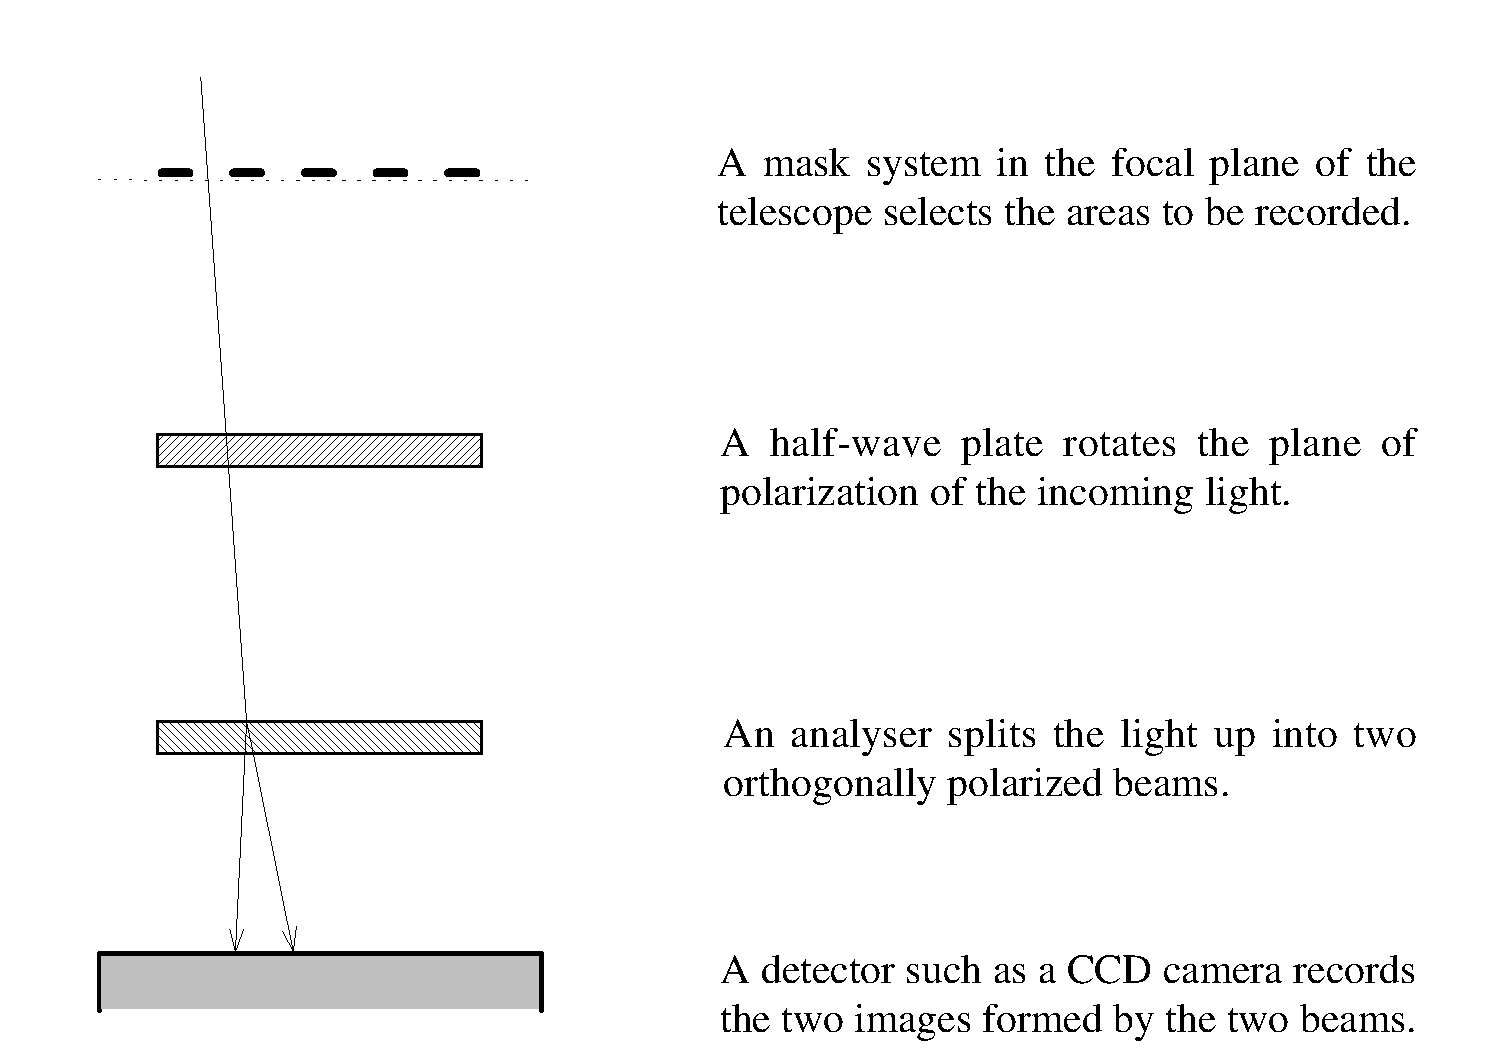
\includegraphics[scale=0.5]{sun223_figures/optical.eps}
  \caption{The main optical components in a typical dual-beam imaging polarimeter.}
  \label{fig:optical}
  \end{center}
  \end{figure}
\end{latexonly}
\begin{htmlonly}
   \begin{quote}
   \begin{figure}[bhtp]
   \label{fig:optical}
   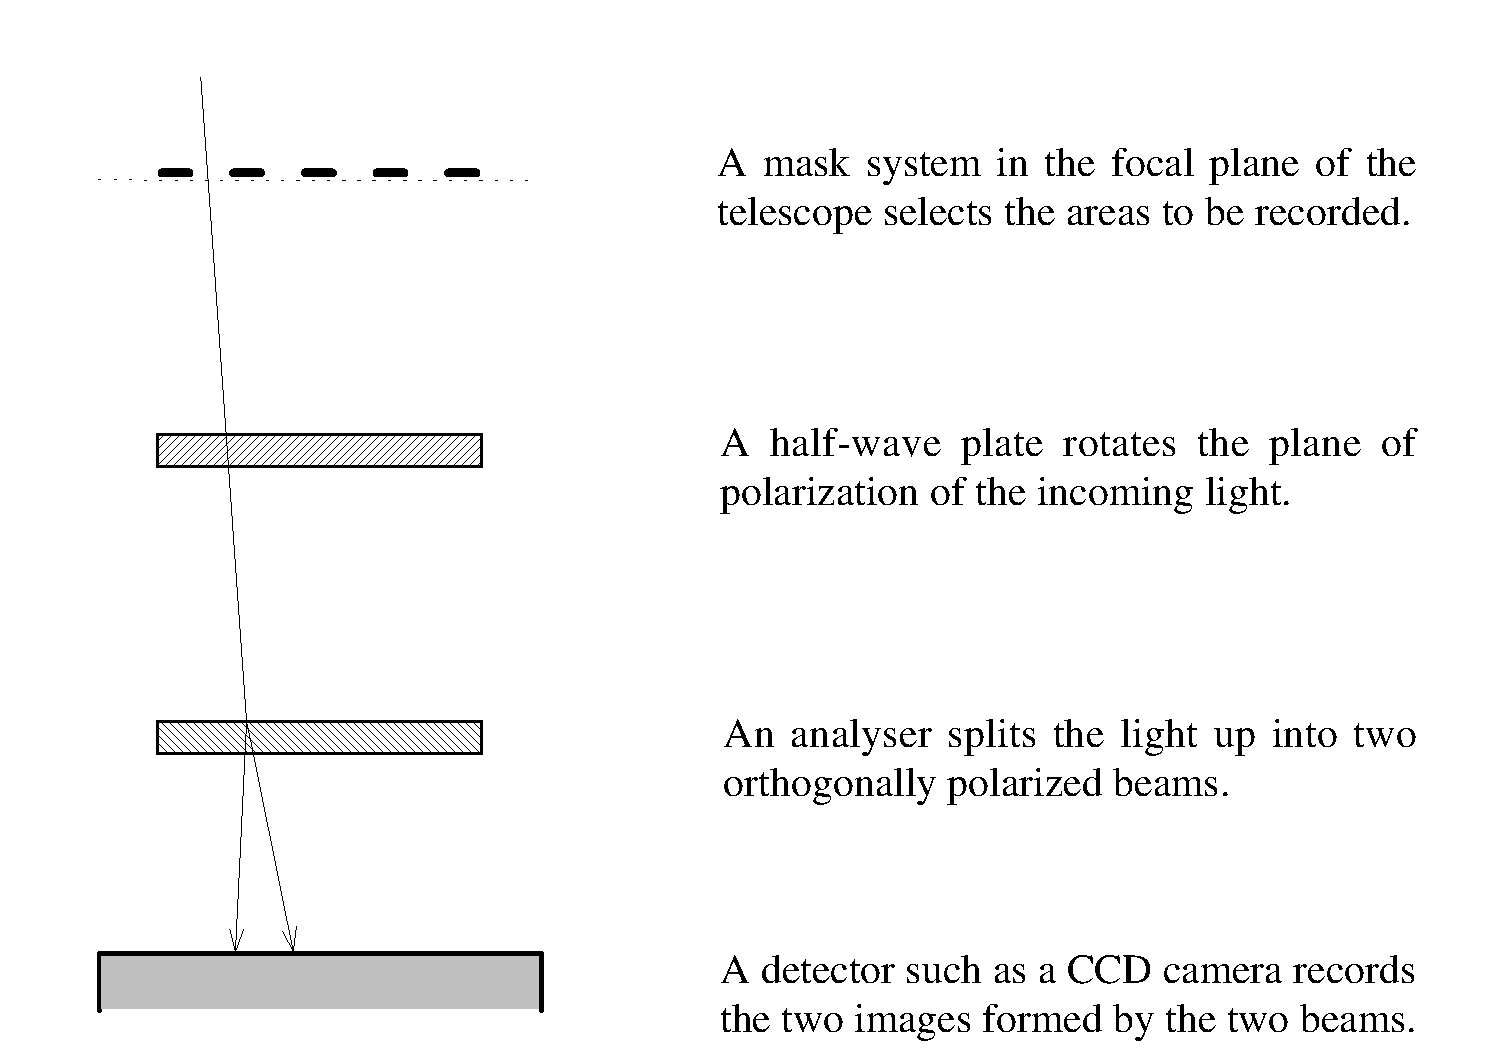
\includegraphics[scale=0.8,width=8in]{sun223_figures/optical.eps}
   \caption{The main optical components in a typical dual-beam imaging polarimeter.}
   \end{figure}
   \end{quote}
\end{htmlonly}

The heart of the polarimeter is the {\em analyser}, which splits incoming
partially plane polarized light up into two beams; one (called the
ordinary, or $O$ ray) contains the component of the incoming light
which is polarized parallel to the axis of the analyser, and the other
(called the extraordinary, or $E$ ray) contains the component of the
incoming light which is polarized orthogonally to the axis of the
analyser. These two beams are recorded simultaneously on a suitable
detector such as a CCD. The advantage of this system over a single-beam
instrument (in which only one state of polarization is recorded on a
given exposure), is that variations in sky background between exposures
affect both states of polarization equally, and so can be eliminated.

In an imaging polarimeter, the two beams form two images on the detector,
displaced by some distance determined by the design of the instrument;
both images representing the same area of the sky. A {\em masking system}
is used to prevent any overlap between the two images. In some
instruments this takes the form of a series of parallel, equally spaced
bars in the focal plane of the telescope (see Figure~\ref{fig:grids}). In
this case, the instrument is designed so that the displacement between
the two images formed by the $O$ and $E$ rays is perpendicular to the
bars, and equal in size to the width of a bar. Thus, the two images form
two inter-leaving sets of bars. There are several other systems (such as 
a mask containing only a single aperture), but the principle is the same.

\begin{latexonly}
  \begin{figure}[p]
  \begin{center}
  \includegraphics[scale=0.8]{sun223_figures/grids.eps}
  \caption{An example of a masking system used in a dual-beam imaging polarimeter.}
  \label{fig:grids}
  \end{center}
  \end{figure}
\end{latexonly}
\begin{htmlonly}
   \begin{quote}
   \begin{figure}[hbtp]
   \label{fig:grids}
   \includegraphics[scale=0.5,width=8in]{sun223_figures/grids.eps}
   \caption{An example of a masking system used in a dual-beam imaging polarimeter.}
   \end{figure}
   \end{quote}
\end{htmlonly}

If the incoming light is only partially polarized, then at least two
exposures are required to estimate both the degree and the orientation of
the polarization, each exposure recording the intensity in two orthogonal
states of polarization as described above. The analyser axis is rotated
in steps of 45\dgs\ between these exposures. In practice, physically rotating
the analyser would result in the displacement between the $O$ and
the $E$ ray images also rotating. This would cause the images to overlap
on the detector and would make the data reduction process much harder (if
not impossible). For this reason, the analyser is usually left in a fixed
position, and the plane of polarization of the incoming light is rotated
instead. This is achieved by placing a {\em half-wave plate} in
front of the analyser, and rotating it in steps of 22.5\dgs, resulting in
a rotation of the plane of polarization of 45\dgs. Using this scheme the
positions of the $O$ and $E$ ray images on the detector are unchanged.

The orientation of the plane of polarization of the incoming light is
measured relative to a fixed ``reference'' direction. The analyser axis
and the 0\dgs\ position of the half-wave plate are usually parallel to
this direction. 

\subsection{\label{SEC:OBS}\xlabel{theobservationalprocedure}The Observational Procedure}
At least two exposures are required to estimate the degree and
orientation of the polarization, taken with half-wave plate positions of
0\dgs\ and 22.5\dgs (see \hyperref{here}{appendix }{}{APP:POL}). For ease
of reference, these exposures are referred to here as $T_{0}$ and
$T_{22.5}$. The $O$ and $E$ ray images in $T_{0}$ measure the intensities
parallel and perpendicular to the reference direction. $T_{22.5}$ has an
effective analyser angle of 45\dgs\ (twice the half-wave plate angle) and
so measures the intensities at angles of 45\dgs\ and 135\dgs\ to the
reference direction

Ideally a further two exposures should be taken at half-wave plate
positions of 45\dgs\ and 67.5\dgs\ (referred to here as exposures
$T_{45}$ and $T_{67.5}$). These provide some redundancy in the data and 
enable internal consistency checks to be made during the data reduction
stage. 

These exposures are denoted by the letter $T$ to indicate that they are
{\em target} exposures. In addition to these target exposures, some {\em
flat-field} exposures are also required. These are used to correct for
any spatial variation in the sensitivity of the system, and consist of
exposures of a photometrically flat surface. Ideally, the flat-field
source should be unpolarized. However, if the additional target exposures
$T_{45}$ and $T_{67.5}$ are taken, then a constant polarization across
the flat-field source can be corrected for during data reduction.

Flat-field exposures should be taken at half-wave plate positions of
0\dgs\ and 22.5\dgs\, and are referred to here as exposures $L_{0}$ and 
$L_{22.5}$. {\em Note, flat-fields are not required for half-wave plate
positions 45\dgs\ and 67.5\dgs\ even if the additional target exposures
$T_{45}$ and $T_{67.5}$ are taken}. Further discussion of the flat-fielding
procedure is given \hyperref{here}{in section }{}{SEC:DETCOR}.

\subsection{The Data Reduction}
Several steps are involved in the production of a polarization map from
the raw exposures recorded by the detector. An over-view of these steps
is given here. Details of how they may be implemented in practice using
POLPACK are given in later sections of this document.

\subsubsection{\label{SEC:DETCOR}Corrections Related to the Detector}
These convert the raw data numbers measured by the detector into values
which are proportional to the combined sky and object intensity
transmitted by the analyser (plus noise of course). The details of these
corrections will depend on the nature of the detector. For a CCD camera,
they will usually involve at least flat-fielding, and de-biassing. 

Flat-fielding is worthy of some extra discussion, since it can be
complicated by the presence of the polarimeter in the light path. The
purpose of flat-fielding is to ensure that there are no spatial
variations in the sensitivity of the detector. This is normally achieved
by taking images of a photometrically flat surface such as the inside of
the observatory dome, or the twilight sky. Since the brightness of this
surface is constant, any variations in the recorded image (the
``flat-field'' image) must be due to variations in the sensitivity of the
detector. These variations can then removed from the target observation
by dividing every pixel value in the target image by the corresponding 
pixel value in the flat-field image.

Introducing a polarimeter into the light path can complicate this if the
flat-field is taken in polarized light (such as produced by reflective
surfaces in the dome, or by light scattering in the atmosphere). In this
case the intensity of the light reaching the detector will not be
constant across the field, but will depend on the polarization. Also, if
the detector itself is intrinsically sensitive to the polarization of
the incident light, then this will introduce a difference in sensitivity
between the two channels.

If the polarization of the flat-field and the polarization-dependency 
of the detector are spatially constant, then the following method for
flat-field correction can be used so long as the additional target
exposures \hyperref{$T_{45}$ and $T_{67.5}$}{$T_{45}$ and $T_{67.5}$ 
(see section }{)}{SEC:OBS} are available:

\begin{enumerate}

\item Divide the two target exposures $T_{0}$ and $T_{45}$ by the flat-field
exposure $L_{0}$.

\item Divide the two target exposures $T_{22.5}$ and $T_{67.5}$ by the 
flat-field exposure $L_{22.5}$.

\end{enumerate}

If this procedure is followed, any constant polarization in the
flat-field source appears as a simple difference in sensitivity between
the two channels of the polarimeter (the ``F-factor''), which can be
estimated and corrected for when calculating the Stokes parameters.
A mathematical description of the flat-fielding and F-factor corrections
is given \hyperref{here}{in appendix }{}{APP:FFCOR}.

\subsubsection{Extraction of the $O$ and $E$ Ray Images}
Each exposure contains two images of the same area of the sky; the $O$
and the $E$ ray images. Once any detector corrections have been applied,
these images need to be identified and extracted into two separate arrays for
further processing.

\begin{latexonly}
  \begin{figure}[htbp]
  \begin{center}
  \includegraphics[scale=0.5]{sun223_figures/extract.eps}
  \caption{Extraction of the $O$ and $E$ ray images.}
  \label{fig:extract}
  \end{center}
  \end{figure}
\end{latexonly}
\begin{htmlonly}
   \begin{quote}
   \begin{figure}[hbtp]
   \label{fig:extract}
   \includegraphics[scale=0.8,width=8in]{sun223_figures/extract.eps}
   \caption{Extraction of the $O$ and $E$ ray images.}
   \end{figure}
   \end{quote}
\end{htmlonly}

\subsubsection{Image Alignment}
The arrays holding the extracted $O$ and $E$ ray images now need to be
aligned so that the same pixel in each array corresponds to the same
position on the sky. This can usually be achieved by aligning stars
within the arrays.

\subsubsection{Sky Subtraction}
The intensity of the background night sky now needs to be estimated and
subtracted from each of the aligned arrays. The sky may be polarized, and
so this needs to be performed independently within each of the aligned arrays.

\subsubsection{Estimation of the Stokes Parameters}
The {\em Stokes parameters} $I$, $Q$ and $U$ are all measures of intensity,
and together provide a useful description of the polarization of the object
being studied. Since $I$, $Q$ and $U$ all have the same units, this
description is generally easier to use than the more obvious description
given by the degree of polarization and the orientation of the plane of
polarization. The mathematical connection between the Stokes parameters 
and the sky-subtracted intensities is described \hyperref{here}{in
appendix }{}{APP:POL}. The output from this stage of the reduction process
is a {\em Stokes vector} (i.e. a set of $I$, $Q$ and $U$ values) for each
measured pixel on the sky.

\subsubsection{Binning of the Stokes Parameters}
One consequence of the fact that the Stokes parameters $I$, $Q$ and $U$
are all measures of intensity, is that they can be binned spatially. This
not only produces less confusing polarization maps (due to the reduced
number of measurements), but also improves the signal-to-noise ratio.

\subsubsection{Calculation of the Degree and Orientation of the Polarization}
The use of Stokes parameters to describe polarization has mathematical
advantages, but is not easy to represent in a graphical manner. For human
interpretation therefore, polarization is usually described by the degree
of polarization, $p$, (i.e. the ratio of polarized to total intensity),
and the orientation of the plane of polarization, $\theta$. Note,
$\theta$ is the angle between the plane of polarization and the reference
direction of the polarimeter. To convert this to a position angle on the
sky, the position angle of the reference direction must be known. The
simplest way to derive these parameters from the Stokes parameters is as
follows:

\begin{myquote}
\begin{eqnarray*}
  I_{p} & = & \sqrt{ Q^{2} + U^{2} } \\
  p & = & I_{p}/I \\ \\
  \theta & = & 0.5.\arctan U/Q
\end{eqnarray*}
\end{myquote}

where $I_{p}$ is the {\em polarized intensity}. However, the estimation
of $p$ is complicated by the non-symmetric statistics produced by squaring
and adding $Q$ and $U$. For low polarizations, this will tend to shift
the mean of the distribution of $p$ to higher values, thus resulting in
an over-estimation of $p$. The use of the following expression for $I_{p}$
reduces the effect of this statistical bias:

\begin{myquote}
\begin{eqnarray*}
  I_{p} & = & \sqrt{ Q^{2} + U^{2} - \sigma^{2}} \\
\end{eqnarray*}
\end{myquote}

where $\sigma^{2}$ is the variance on $Q$ or $U$ (which are assumed
equal). A description of the statistical behaviour of polarization
parameters is given by Serkowski ({\em Advances in Astronomy and
Astrophysics}, ed. Z. Kopal, Academic Press, New York, London (1962),
{\bf 1}, 304).

\subsubsection{Display of the Final Polarization Data}
The final polarization parameters are usually presented graphically in
the form of a {\em polarization map}. Each measurement is represented as
a vector parallel to the plane of polarization. The length of the vector
is proportional to the degree of polarization, which varies from 0\% to
100\%. The Stokes vectors can be binned to reduce the number of vectors
in the map to a manageable number. The map is often overlayed on a total
intensity image of the object to emphasize any correlation between the
visual appearance of the object and the morphology of the polarization
map.

\section{\xlabel{datareductionusingpolpack}Data Reduction Using POLPACK}


\section{\xlabel{startup}Starting up POLPACK}

The applications within POLPACK are made available from the C shell using the 
command:
\begin{myquote}
\begin{verbatim}
% polpack
\end{verbatim}
\end{myquote}

Note that the \text{\%} represents the C-shell prompt and should not be typed.
POLPACK is also available from the \xref{ICL}{sg5}{} command language.

\subsection{\xlabel{gettinghelp}Getting Help}

Help is available in several forms: 
\begin{itemize}
\item As simple text in the command-line window. Type:

\begin{myquote}
\begin{verbatim}
% polhelp
\end{verbatim}
\end{myquote}

Additional arguments may be given indicating the subject on which help is
required. For instance:

\begin{myquote}
\begin{verbatim}
% polhelp polka parameters
\end{verbatim}
\end{myquote}

will enter the help library at the point containing information on the
parameters available for application POLKA.

\item As hypertext in a separate browser window. Type:

\begin{myquote}
\begin{verbatim}
% showme sun223
\end{verbatim}
\end{myquote}

\item In response to prompts issued by applications for parameter values. 
Entering a single question mark will display help on the parameter being
prompted for, and then return you to the parameter prompt. Entering two
question marks also displays help on the parameter, but will leave you in the
help library, allowing you to navigate through any other necessary
topics. Leaving the help library returns you to the parameter prompt.

\item Additional information describing the detailed use of the POLKA
GUI is available from the {\em Help} menu within the GUI.

\end{itemize}

\subsection{Running from the C-shell}
When using POLPACK from the C-shell (or any other shell) care needs to be
taken with some special characters. Wildcard characters \text{*,?,[a-z]},
quoted strings \text{""} and vector braces \text{[ ]} must be protected
by using either the escape character {\small \verb+\+} or by single
quotes (wildcard characters must be protected as these are expanded
internally by POLPACK, rather than by the shell).

\section{POLPACK's data format}
POLPACK uses data stored in the NDF format (the N-dimensional data
format (\xref{SUN/33}{sun33}{}), which is based on HDS,
the Hierarchical Data System \xref{(SUN/92)}{sun92}{}).
This is portable between the operating
systems that POLPACK runs on (Digital UNIX, Solaris and Linux at this time)
so it can be copied, accessed via NFS and ftp'd (using binary
transfer) between these systems. If your data is in another format you
will need to convert it to NDF. The CONVERT package
(\xref{SUN/55}{sun55}{}) contains many applications for doing this. The
KAPPA package (\xref{SUN/95}{sun95}{}) contains an application
\xref{FITSIN}{sun95}{FITSIN} that reads FITS tapes and writes the
results as NDFs.

\newpage
\appendix
\section{Description of the POLPACK applications \label{app:description}}
\begin{latexonly}
\latexonlysubsection{Alphabetic list of POLPACK routines.}
%
% set up a mini table of contents for this section pointing into next section.
%
\quickdes{POLBIN}{Bins a catalogue containing Stokes vectors.}{ POLBIN }

\quickdes{POLCAL}{Calculates Stokes vectors from a set of aligned intensity images.}{ POLCAL }

\quickdes{POLEXP}{Exports POLPACK information within an NDF to a FITS extension.}{ POLEXP }

\quickdes{POLIMP}{Imports POLPACK information into an NDF from a FITS
extension.}{ POLEXP }

\quickdes{POLHELP}{Displays textual help information for POLPACK.}{
POLHELP }

\quickdes{POLKA}{An X-based GUI which converts raw photometric images
into Stokes vectors.}{ POLKA }

\quickdes{POLPLOT}{Displays polarization vectors supplied in a
catalogue.}{ POLPLOT }

\quickdes{POLVEC}{Converts a Stokes vector cube into a catalogue of
polarization vectors.}{ POLVEC }

\end{latexonly}

\subsection{Complete routine descriptions \label{descriptions}}

The POLPACK routine descriptions are contained in the following pages.

% +
%  Name:
%     SST.TEX

%  Purpose:
%     Define LaTeX commands for laying out Starlink routine descriptions.

%  Language:
%     LaTeX

%  Type of Module:
%     LaTeX data file.

%  Description:
%     This file defines LaTeX commands which allow routine documentation
%     produced by the SST application PROLAT to be processed by LaTeX and
%     by LaTeX2html. The contents of this file should be included in the
%     source prior to any statements that make of the sst commnds.

%  Notes:
%     The commands defined in the style file html.sty provided with LaTeX2html
%     are used. These should either be made available by using the appropriate
%     sun.tex (with hypertext extensions) or by putting the file html.sty
%     on your TEXINPUTS path (and including the name as part of the
%     documentstyle declaration).

%  Authors:
%     RFWS: R.F. Warren-Smith (STARLINK)
%     PDRAPER: P.W. Draper (Starlink - Durham University)

%  History:
%     10-SEP-1990 (RFWS):
%        Original version.
%     10-SEP-1990 (RFWS):
%        Added the implementation status section.
%     12-SEP-1990 (RFWS):
%        Added support for the usage section and adjusted various spacings.
%     8-DEC-1994 (PDRAPER):
%        Added support for simplified formatting using LaTeX2html.
%     {enter_further_changes_here}

%  Bugs:
%     {note_any_bugs_here}

% -

%  Define length variables.
\newlength{\sstbannerlength}
\newlength{\sstcaptionlength}
\newlength{\sstexampleslength}
\newlength{\sstexampleswidth}

%  Define a \tt font of the required size.
\newfont{\ssttt} {cmtt10 scaled 1095}

%  Define a command to produce a routine header, including its name,
%  a purpose description and the rest of the routine's documentation.
\newcommand{\sstroutine}[3]{
   \newpage
   \label{#1}
   \goodbreak
   \rule{\textwidth} {0.5mm}
   \vspace{-7ex}
   \newline
   \settowidth{\sstbannerlength} {{\Large {\bf #1}}}
   \setlength{\sstcaptionlength} {\textwidth}
   \setlength{\sstexampleslength} {\textwidth}
   \addtolength{\sstbannerlength} {0.5em}
   \addtolength{\sstcaptionlength} {-2.0\sstbannerlength}
   \addtolength{\sstcaptionlength} {-5.0pt}
   \settowidth{\sstexampleswidth} {{\bf Examples:}}
   \addtolength{\sstexampleslength} {-\sstexampleswidth}
   \parbox[t]{\sstbannerlength} {\flushleft{\Large {\bf #1}}}
   \parbox[t]{\sstcaptionlength} {\center{\Large #2}}
   \parbox[t]{\sstbannerlength} {\flushright{\Large {\bf #1}}}
   \begin{description}
      #3
   \end{description}
}

%  Format the description section.
\newcommand{\sstdescription}[1]{\item[Description:] #1}

%  Format the usage section.
\newcommand{\sstusage}[1]{\item[Usage:] \mbox{}
   \begin{description}
      {\ssttt \item #1}
   \end{description}
}

%  Format the invocation section.
\newcommand{\sstinvocation}[1]{\sloppy \item[Invocation:]\hspace{0.4em} {\tt #1}}

%  Format the arguments section.
\newcommand{\sstarguments}[1]{
   \item[Arguments:] \mbox{} \\
   \vspace{-3.5ex}
   \begin{description}
      #1
   \end{description}
}

%  Format the returned value section (for a function).
\newcommand{\sstreturnedvalue}[1]{
   \item[Returned Value:] \mbox{} \\
   \vspace{-3.5ex}
   \begin{description}
      #1
   \end{description}
}

%  Format the parameters section (for an application).
\newcommand{\sstparameters}[1]{
   \item[Parameters:] \mbox{} \\
   \vspace{-3.5ex}
   \begin{description}
      #1
   \end{description}
}

%  Format the examples section.
\newcommand{\sstexamples}[1]{
   \item[Examples:] \mbox{} \\
   \vspace{-3.5ex}
   \begin{description}
      #1
   \end{description}
}

%  Define the format of a subsection in a normal section.
\newcommand{\sstsubsection}[1]{ \item[{#1}] \mbox{} \\}

%  Define the format of a subsection in the examples section.
\newcommand{\sstexamplesubsection}[2]{\sloppy \item{\ssttt #1} \mbox{} \\ #2 }

%  Format the notes section.
\newcommand{\sstnotes}[1]{\item[Notes:] \mbox{} \\[1.3ex] #1}

%  Provide a general-purpose format for additional (DIY) sections.
%\newcommand{\sstdiytopic}[2]{\item[{\hspace{-0.35em}#1\hspace{-0.35em}:}] \mbox{} \\[1.3ex] #2}
\newcommand{\sstdiytopic}[2]{\item[#1:] \mbox{} \\[1.3ex] #2}

%  Format the implementation status section.
\newcommand{\sstimplementationstatus}[1]{
   \item[{Implementation Status:}] \mbox{} \\[1.3ex] #1
}

%  Format the bugs section.
\newcommand{\sstbugs}[1]{\item[Bugs:] #1}

%  Format a list of items while in paragraph mode.
\newcommand{\sstitemlist}[1]{
  \mbox{} \\
  \vspace{-3.5ex}
  \begin{itemize}
     #1
  \end{itemize}
}

%  Define the format of an item.
\newcommand{\sstitem} {\item}

%  Now define html equivalents of those already set. These are used by
%  latex2html and are defined in the html.sty files.
\begin{htmlonly}

%  Re-define \ssttt.
   \newcommand{\ssttt} {\tt}

%  sstroutine.
   \renewcommand{\sstroutine}[3]{
      \subsection{#1\xlabel{#1}-\label{#1}#2}
      \begin{description}
         #3
      \end{description}
   }

%  sstdescription
   \renewcommand{\sstdescription}[1]{\item[Description:]
      \begin{description}
         #1
      \end{description}
   }

%  sstusage
   \renewcommand{\sstusage}[1]{\item[Usage:]
      \begin{description}
         {\ssttt #1}
      \end{description}
   }

%  sstinvocation
   \renewcommand{\sstinvocation}[1]{\item[Invocation:]
      \begin{description}
         {\ssttt #1}
      \end{description}
   }

%  sstarguments
   \renewcommand{\sstarguments}[1]{
      \item[Arguments:]
      \begin{description}
         #1
      \end{description}
   }

%  sstreturnedvalue
   \renewcommand{\sstreturnedvalue}[1]{
      \item[Returned Value:]
      \begin{description}
         #1
      \end{description}
   }

%  sstparameters
   \renewcommand{\sstparameters}[1]{
      \item[Parameters:]
      \begin{description}
         #1
      \end{description}
   }

%  sstexamples
   \renewcommand{\sstexamples}[1]{
      \item[Examples:]
      \begin{description}
         #1
      \end{description}
   }

%  sstsubsection
   \renewcommand{\sstsubsection}[1]{\item[{#1}]}

%  sstexamplesubsection
   \renewcommand{\sstexamplesubsection}[2]{\item[{\ssttt #1}] \\ #2}

%  sstnotes
   \renewcommand{\sstnotes}[1]{\item[Notes:]
      \begin{description}
         #1
      \end{description}
   }

%  sstdiytopic
   \renewcommand{\sstdiytopic}[2]{\item[{#1}]
      \begin{description}
         #2
      \end{description}
   }

%  sstimplementationstatus
   \renewcommand{\sstimplementationstatus}[1]{\item[Implementation Status:]
      \begin{description}
         #1
      \end{description}
   }

%  sstitemlist
   \newcommand{\sstitemlist}[1]{
      \begin{itemize}
         #1
      \end{itemize}
   }
\end{htmlonly}

%  End of "sst.tex" layout definitions.
% .
% -----------------------------------------------------------------------------

\newpage
\sstroutine{
   POLBIN
}{
   Bins a catalogue containing Stokes vectors
}{
   \sstdescription{
      This application creates a new catalogue of polarization vectors by
      binning the Stokes vectors in the supplied catalogue. The input
      catalogue should contain columns with the same names and meanings
      as those produced by POLVEC. In particularly, the bin sizes are
      given as increments within the coordinate Frame implied by the
      columns with names {\tt "}X{\tt "} and {\tt "}Y{\tt "}. If the original catalogue was
      created by POLVEC, then {\tt "}X{\tt "} and {\tt "}Y{\tt "} will be pixel coordinates within
      the cube supplied as input to POLVEC.

      The bins used form a grid of equal sized rectangular cells, the
      dimensions of each cell being specified by the user. The grid contains
      sufficient cells to span the entire range of X and Y covered by the
      input catalogue. Each position in the output catalogue corresponds
      to one of these cells. The Stokes parameters for the cell are formed
      by combining together the Stokes parameter of all input positions
      which fall within the cell, using a method specified by the user.
      The degree of polarization, angle of polarization, and polarized
      intensity are then derived from these Stokes parameters. The (X,Y)
      positions in the output catalogue are the positions at the centre
      of each of the cells.
   }
   \sstusage{
      polbin in out box [method]
   }
   \sstparameters{
      \sstsubsection{
         BOX( 2 ) = \_REAL (Read)
      }{
         The x and y bin sizes (in pixels). These values refer to the
         coordinate Frame defined by columns {\tt "}X{\tt "} and {\tt "}Y{\tt "}.
      }
      \sstsubsection{
         DEBIAS = \_LOGICAL (Read)
      }{
         TRUE if a correction for statistical bias is to be made to
         percentage polarization and polarized intensity. This correction
         subtracts the variance of the percentage polarization from the
         squared percentage polarization, and uses the square root of this
         as the corrected percentage polarization.  The corresponding
         polarized intensity is then found by multiplying the corrected
         percentage polarization by the total intensity.  The returned
         variance values are unchanged. This correction only applies to
         calculations of plane polarization, and cannot be used if the
         input catalogue does not contain variance values. If a null value
         (!) is supplied, then the correction is applied if output variances
         are being created, and not otherwise.           [!]
      }
      \sstsubsection{
         IN = LITERAL (Read)
      }{
         The name of the input catalogue.
      }
      \sstsubsection{
         METHOD = LITERAL (Read)
      }{
         The method to be used when binning Stokes parameters. This may be
         set to any unique abbreviation of the following:
         \sstitemlist{

            \sstitem
               MEAN      -- Mean of the input data values

            \sstitem
               MEDIAN    -- Median of the input data values

            \sstitem
               SIGMA     -- A sigma clipped mean
            [MEDIAN]
         }
      }
      \sstsubsection{
         MINVAL = \_INTEGER (Read)
      }{
         The minimum number of good input values which must be present in
         a cell to create a good output value. [1]
      }
      \sstsubsection{
         OUT = LITERAL (Read)
      }{
         The name of the output catalogue.
      }
      \sstsubsection{
         SIGMAS = \_REAL (Read)
      }{
         Number of standard deviations to reject data at. Only used if
         METHOD is set to {\tt "}SIGMA{\tt "}. [4.0]
      }
   }
   \sstexamples{
      \sstexamplesubsection{
         polbin intab outtab 4
      }{
         Bins the Stokes vectors in catalogue {\tt "}intab{\tt "} and produces
         catalogue {\tt "}outtab{\tt "} containing binned Stokes parameters and
         corresponding polarization parameters. Each bin measures 4 units
         along both the X and Y axes, and has a value based on the median
         of the corresponding input Stokes values.
      }
   }
}
\sstroutine{
   POLCAL
}{
   Calculate polarization parameters for dual-beam imaging
   linear and circular polarimetry
}{
   \sstdescription{
      Calculate polarization parameters for dual-beam imaging
      polarimetry. This routine accesses a list of input NDF data
      structures which should contain processed polarimetric
      information. It is assumed that the input data are bias/dark
      corrected, flatfielded, sky subtracted and mutually aligned.

      Each input NDF should contain an image recorded in a
      single polarization state. The polarization state should be
      indicated by two descriptors WPLATE (the waveplate position, one of
      0.0,45.0,22.5,67.5) and RAY (either O (ordinary) or E
      (extraordinary)) which should reside in a POLPACK NDF extension.
      The descriptors are checked for validity and used to sort the
      input data into polarimetric sets. In addition, a third
      descriptor, IMGID, should be present to indicate which images were
      recorded on the same exposure.

      The input data files are first validated using the descriptor
      information in their POLPACK extensions. They are then sorted into
      sets that can be used to calculate the output polarization
      parameters.

      The instrumental polarization efficiency (F factor) is calculated
      by intercomparing images to calculate the scale factors and zero
      levels. All possible intercomparisons are used and a weighted mean
      F factor calculated.

      The time dependent efficiencies (E factors) due, for example, to
      changes in integration time or sky conditions between exposures,
      are calculated. The E factors are calculated by comparing total
      intensity images against an iteratively refined median image.

      The input data is `corrected{\tt '} by the polarization and time
      dependent efficiencies and the stokes images (I,Q,U) or (I,V) are
      calculated. The output stokes images are formed by median stacking
      all possible estimates.

      In LINEAR polarimetry mode the output NDF contains I, Q and U
      stokes images. In CIRCULAR polarimetry mode the output NDF
      contains I, V stokes images.
   }
}
\sstroutine{
   POLEXP
}{
   Copies information from the POLPACK extension to the FITS extension
}{
   \sstdescription{
      This routine creates FITS header cards describing the contents of
      the POLPACK extensions in a group of NDFs. The header cards are
      written to the FITS extensions of the NDFs, replacing any existing
      cards for the same keywords. The keywords used are listed below.
      Information exported to the FITS extension can be imported back
      into the POLPACK extension using POLIMP.

      The main use of this routine is for exporting POLPACK NDFs for use
      bu other non-NDF based packages.
   }
   \sstusage{
      POLEXP in
   }
   \sstparameters{
      \sstsubsection{
         IN = LITERAL (Read)
      }{
         A list of NDF names. The NDF names should be separated by commas
         and may include wildcards.
      }
      \sstsubsection{
         NAMELIST = LITERAL (Read)
      }{
         The name of a file to create containing a list of the
         succesfully processed NDFs. This file can be used when
         specifying the input NDFs for subsequent applications. [!]
      }
      \sstsubsection{
         QUIET = \_LOGICAL (Read)
      }{
         If FALSE, then each NDF is listed as it is processed. Otherwise,
         nothing is written to the screen. [FALSE]
      }
   }
   \sstexamples{
      \sstexamplesubsection{
         POLEXP in=$\wedge$names.lis
      }{
         This example processes the NDFs listed in the text file
         {\tt "}names.lis{\tt "}. The information stored in the POLPACK extension of
         each is exported to the FITS extension.
      }
   }
   \sstdiytopic{
      FITS Keywords
   }{
      The following FITS keywords are created. The POLPACK extension item
      stored in the keyword is shown in parenthesise (see POLIMP for a
      description of these extension items):

            PPCKANGR  (ANGROT)
            PPCKFILT  (FILTER)
            PPCKIMID  (IMGID)
            PPCKWPLT  (WPLATE)
            PPCKRAY   (RAY)
            PPCKROT   (ROTATION)
            PPCKYROT  (YROTATION)
            PPCKSTOK  (STOKES)
   }
}
\sstroutine{
   POLHELP
}{
   Gives help about POLPACK
}{
   \sstdescription{
      Displays help about POLPACK.  The help information has
      alphabetical lists of commands, general information about
      POLPACK and related material; it describes individual commands in
      detail.

      Here are some of the main options.
         polhelp
            No parameter is given so the introduction and the top-level
            help index is displayed.
         polhelp application/topic
            This gives help about the specified application or topic.
         polhelp application/topic subtopic
            This lists help about a subtopic of the specified
            application or topic. The hierarchy of topics has a maximum
            of four levels.

      See the Section {\tt "}Navigating the Help Library{\tt "} for details how to
      move around the help information, and to select the topics you
      want to view.
   }
   \sstusage{
      polhelp [topic] [subtopic] [subsubtopic] [subsubsubtopic]
   }
   \sstparameters{
      \sstsubsection{
         TOPIC = LITERAL (Read)
      }{
         Topic for which help is to be given. [{\tt "} {\tt "}]
      }
      \sstsubsection{
         SUBTOPIC = LITERAL (Read)
      }{
         Subtopic for which help is to be given. [{\tt "} {\tt "}]
      }
      \sstsubsection{
         SUBSUBTOPIC = LITERAL (Read)
      }{
         Subsubtopic for which help is to be given. [{\tt "} {\tt "}]
      }
      \sstsubsection{
         SUBSUBSUBTOPIC = LITERAL (Read)
      }{
         Subsubsubtopic for which help is to be given. [{\tt "} {\tt "}]
      }
   }
   \sstdiytopic{
      Navigating the Help Library
   }{
      The help information is arranged hierarchically.  You can move
      around the help information whenever POLHELP prompts.  This
      occurs when it has either presented a screen{\tt '}s worth of text or
      has completed displaying the previously requested help.  The
      information displayed by POLHELP on a particular topic includes a
      description of the topic and a list of subtopics that further
      describe the topic.

      At a prompt you may enter:
         o  a topic and/or subtopic name(s) to display the help for that
            topic or subtopic, so for example, {\tt "}polka parameters dpi{\tt "}
            gives help on DPI, which is a subtopic of Parameters, which
            in turn is a subtopic of POLKA;

         o  a $<$CR$>$ to see more text at a {\tt "}Press RETURN to continue ...{\tt "}
            request;

         o  a $<$CR$>$\} at topic and subtopic prompts to move up one level
            in the hierarchy, and if you are at the top level it will
            terminate the help session;

         o  a CTRL/D (pressing the CTRL and D keys simultaneously) in
            response to any prompt will terminate the help session;

         o  a question mark {\tt "}?{\tt "} to redisplay the text for the current
            topic, including the list of topic or subtopic names; or

         o  an ellipsis {\tt "}...{\tt "} to display all the text below the
            current point in the hierarchy.  For example, {\tt "}POLKA...{\tt "}
            displays information on the POLKA topic as well as
            information on all the subtopics under POLKA.

      You can abbreviate any topic or subtopic using the following
      rules.

         o  Just give the first few characters, e.g. {\tt "}PARA{\tt "} for
            Parameters.

         o  Some topics are composed of several words separated by
            underscores.  Each word of the keyword may be abbreviated,
            e.g. {\tt "}Colour\_Set{\tt "} can be shortened to {\tt "}C\_S{\tt "}.

         o  The characters {\tt "}\%{\tt "} and {\tt "}$*${\tt "} act as wildcards, where the
            percent sign matches any single character, and asterisk
            matches any sequence of characters.  Thus to display
            information on all available topics, type an asterisk in
            reply to a prompt.

         o  If a word contains, but does end with an asterisk wildcard,
            it must not be truncated.

         o  The entered string must not contain leading or embedded
            spaces.

      Ambiguous abbreviations result in all matches being displayed.
   }
   \sstimplementationstatus{
      \sstitemlist{

         \sstitem
         Uses the portable help system.
      }
   }
}
\sstroutine{
   POLIMP
}{
   Stores information in the POLPACK extension
}{
   \sstdescription{
      This routine should be used to prepare data prior to processing
      with POLPACK. It records the values of various items of information
      required by POLPACK (wave-plate position, filter, etc) in the POLPACK
      extensions of the supplied NDFs. These values can either be supplied
      explicitly or can be copied ({\tt "}imported{\tt "}) from keywords stored in the
      FITS extensions of the supplied NDFs. Such keywords may, for instance,
      be provided by the instrument/telescope control systems.

      The import is controlled by a {\tt "}table{\tt "} which specifies how FITS
      keyword values should be used to create the corresponding POLPACK
      extension items. Each extension item may be assigned a specified
      constant value, the value of a specified FITS keyword, or the value
      of an arbitrary function of several FITS keywords.

      During the processing of data, POLPACK adds items to the POLPACK
      extension to indicate the state of the processing which has been
      applied to the data. This routine also allows values to be assigned
      to these extra extension items and thus can be used to import partially
      processed data. POLIMP can be used in conjunction with POLEXP to
      allow data to be moved backwards and forwards between POLPACK and
      other non-NDF based packages.
   }
   \sstusage{
      polimp in table
   }
   \sstparameters{
      \sstsubsection{
         IN = LITERAL (Read)
      }{
         A list of NDF names. The NDF names should be separated by commas
         and may include wildcards.
      }
      \sstsubsection{
         NAMELIST = LITERAL (Read)
      }{
         The name of a file to create containing a list of the
         succesfully processed NDFs. This file can be used when
         specifying the input NDFs for subsequent applications. [!]
      }
      \sstsubsection{
         QUIET = \_LOGICAL (Read)
      }{
         If FALSE, then the values stored in each NDF are listed as it is
         processed. Otherwise, nothing is written to the screen. [FALSE]
      }
      \sstsubsection{
         TABLE = LITERAL (Read)
      }{
         The name of the file containing the table describing how FITS
         keyword values are to be translated into POLPACK extension
         items. See the topic {\tt "}Table Format{\tt "} for information on how to
         create a translation table. If a null value (!) is supplied,
         then a default table is used which corresponds to the FITS
         keywords written by POLEXP:

            ANGROT      PPCKANGR
            FILTER      PPCKFILT
            IMGID       PPCKIMID
            WPLATE      PPCKWPLT
            RAY?        PPCKRAY
            ROTATION?   PPCKROT
            YROTATION?  PPCKYROT
            STOKES?     PPCKSTOK
         [!]
      }
   }
   \sstexamples{
      \sstexamplesubsection{
         polimp in={\tt '}$*${\tt '} table=mytable.dat
      }{
         This example processes all the NDFs in the current directory
         using the import control table mytable.dat.
      }
      \sstexamplesubsection{
         polimp in=$\wedge$names.lis
      }{
         This example processes the NDFs listed in the text file
         {\tt "}names.lis{\tt "} using the default control table appropriate for
         partially processed data which has previously been exported using
         POLEXP.
      }
   }
   \sstnotes{
      \sstitemlist{

         \sstitem
         Any existing values in the POLPACK extension are deleted before
         processing the supplied control table.

         \sstitem
         A new Frame is added to the NDF{\tt '}s WCS component and is given the
         Domain {\tt "}POLANAL{\tt "}. This Frame is formed by rotating the pixel coordinates
         Frame so that the first axis is parallel to the analyser axis. The
         angle of rotation is given by the ANGROT item in the POLPACK extension
         and defaults to zero if ANGROT is not specified in the control table.
      }
   }
   \sstdiytopic{
      Table Format
   }{
      The import control (translation) table is an ordinary text file
      which contains instructions on how to assign values to the components
      of the POLPACK extension in an NDF. Constant values specified in
      the file may be used, or the values may be derived from the values
      of FITS keywords stored in the FITS extension of the NDF.

      In its most simple format each line in a FITS control table contains
      the name of a POLPACK extension item, followed by a constant value
      or FITS keyword. This causes the value of the specified FITS keyword
      or constant, to be assigned to the specified extension item. Some
      examples:

         ANGROT             ANROTA

      This copies the value of the FITS keyword ANROTA from the FITS
      extension to the ANGROT component in the POLPACK extension.

         ANGROT             45.0

      This assigns the value 45.0 to the ANGROT component of the POLPACK
      extension.

         IMGID              {\tt "}M51\_PLATEB{\tt "}

      This assigns the value M51\_PLATE to the IMGID component of the
      POLPACK extension. Note, textual constants must be enclosed within
      quotes.

      In addition to using the values of FITS keywords directly, it is also
      possible to use arbitrary functions of one or more keywords. To do
      this, each keyword used in the function must first be {\tt "}declared{\tt "} so
      that a data type may be associated with it. This is done by including
      lines with the following form in the control table prior to the
      function reference:

         Data-type          FITS-keyword

      Here {\tt "}Data-type{\tt "} must be one of \_INTEGER, \_REAL, \_DOUBLE, \_WORD, \_BYTE,
      \_CHAR. So for instance if you wanted to assign a value to the ANGROT
      extension item, the orientation of the analyser in degrees, from the
      FITS keyword ROTA which gives the required value in radians, you
      could use this sequence of commands:

         \_REAL             ROTA
         ANGROT            57.29578$*$ROTA

      The function may use any of the usual Fortran operators; $+$, -, $*$, /,
      $*$$*$ and built-in functions (SIN, COS, TAN, LOG, etc). See SUN/61
      (appendix A) for complete details.

      Characters strings cannot be manipulated by these functions so a single
      special format for translating their values is provided. The name
      of the destination extension item is given as usual followed by a
      FITS-keyword which supplies the string to be translated. This is then
      followed by statements which translate an {\tt "}input{\tt "} string into an
      {\tt "}output{\tt "} string. So for instance if you wanted to translate waveplate
      positions to the equivalent strings recognised by POLPACK you might
      use something like:

         WPLATE     WAVEPLT  A=0.0 -
                             B=22.5 -
                             C=45.0 -
                             D=67.5

      This does a case insensitive comparison between the value of the FITS
      keyword WAVEPLT and the strings on the left hand sides of the equals
      signs ({\tt "}A{\tt "}, {\tt "}B{\tt "}, etc), If a match is found, it assigns the value from
      the right hand side of the equals sign ({\tt "}0.0{\tt "}, {\tt "}22.5{\tt "}, etc, these
      are interpreted as strings, not numerical values) to the WPLATE
      component in the POLPACK extension. An error is reported if no match
      is found. The {\tt "}-{\tt "} signs at the end of each line indicate that the list
      continues on the next line. Note, if specified FITS keyword has a
      numerical value, then it is converted into textual form before doing
      the comparisons.

      If a control table contains more than one line for an extension
      item, then each line is processed in turn, replacing any value
      established by earlier lines. Thus the final value of the extension
      item will be given by the last line in the table refering to the
      extension item.

      If it is not known in advance if the FITS extension will contain the
      keyword values needed to assign a value to a particular POLPACK
      extension item, then a question mark may be appended to the name of
      the POLPACK extension item. If the required FITS keyword values
      cannot be found, then the error messages which would normally be
      issued are suppressed, and any remaining lines in the control table
      are processed as normal. If no value has been assigned to the item
      when the entire table has been processed, then the item will be set
      to its default value if it has one, or left undefined otherwise (see
      below). For instance:

         RAY?  OLDRAY
         RAY?  PPCKRAY

      causes the POLPACK extension item RAY to be assigned the value of the
      FITS keyword PPCKRAY if the keyword has a value in the FITS
      extension. If not, then the FITS keyword OLDRAY is used instead. If
      this does not exist either, then RAY is left undefined.

      Logical data types are restricted to a single keyword whose value
      must be {\tt "}YES{\tt "}, {\tt "}TRUE{\tt "}, {\tt "}T{\tt "}, {\tt "}Y{\tt "} for TRUE or {\tt "}NO{\tt "}, {\tt "}FALSE{\tt "}, {\tt "}N{\tt "},
      {\tt "}F{\tt "}.

      Fields in the table may be separated by commas if desired, any
      amount of white space and tabs are also allowed. Comments may be
      placed anywhere and should start with the characters {\tt "}\#{\tt "} or {\tt "}!{\tt "}.
      Continuation onto a new line is indicated by use of {\tt "}-{\tt "}.
   }
   \sstdiytopic{
      POLPACK extension items
   }{
      The POLPACK extension of an NDF may contain the following items.
      The names and types of the extension items are those as used in
      import tables. Of these, ANGROT, FILTER, WPLATE and possibly IMGID
      are the only ones that most users need be concerned with. Values
      should be assigned to these extension items before processing of
      raw data commences. Their values will often be derived from FITS
      headers written by the instrument/telescope control system. Values
      for the remaining extension items are produced by POLPACK as the
      processing proceeds and need only be included in the control
      table if you are importing partially processed data.

      Some extension items have default values which are used if the
      control table does not specify a value for them. These are
      indicated in the descriptions below:

         ANGROT (\_REAL):  The anti-clockwise angle from the first axis of
         the image to the analyser position corresponding to WPLATE=0.0,
         in degrees. Defaults to 0.0.

         FILTER (\_CHAR):  The filter name. If a value is supplied, then
         the value of WPLATE is appended to it (unless the filter already
         includes the WPLATE value). This value is also copied to the FILTER
         item in the CCDPACK extension. Defaults to the value of WPLATE.

         IMGID (\_CHAR):  An arbitrary textual identifier for each input
         image, used to associate corresponding O and E ray images. It must
         be unique amongst the input images. Defaults to the name of the
         input image.

         RAY (\_CHAR):  This item should only be specified in the control
         table if the images being imported are partially processed images
         which have been split into separate O and E ray images. It
         identifies which ray the image is derived from, and can take the
         two values {\tt "}O{\tt "} and {\tt "}E{\tt "} (upper case). Left undefined by default.

         ROTATION (\_REAL):  This item should only be specified in the
         control table if the images being imported are partially processed
         images which have already been aligned. It is the clockwise
         rotation introduced into the image in order to align it with other
         images, in degrees. Left undefined by default.

         STOKES (\_CHAR):  This item should only be specified in the
         control table if the images being imported are partially processed
         images containing Stokes parameters. It is a string containing one
         character for each plane in the data array of the NDF. Each
         character identifies the quantity stored in the corresponding plane
         of the data array, and will be one of I, Q, U or V. Left
         undefined by default.

         WPLATE (\_CHAR):  The wave-plate position, in degrees. Must be one
         of; {\tt "}0.0{\tt "}, {\tt "}22.5{\tt "}, {\tt "}45.0{\tt "}, {\tt "}67.5{\tt "}. There is no default (an error
         is reported if no value is supplied).

         YROTATION (\_REAL): This item should only be specified in the
         control table if the images being imported are partially processed
         images which have already been aligned, and if the final map may
         contain shear. It gives the clockwise rotation in degrees of the
         Y axis introduced into the image in order to align it with other
         images. In this case the ROTATION item (see above) is understood
         as giving the rotation of the X axis. Left undefined by default.
   }
}
\sstroutine{
   POLKA
}{
   Extract and align O and E ray areas from a set of images
}{
   \sstdescription{
      This routine extracts and aligns areas containing corresponding rays
      from a set of images containing dual or single beam polarimetry data.
      It can also perform sky subtraction based either on a set of
      supplied sky frames, or on user-specified background areas within
      the object frames.

      In dual-beam mode, two output images are created for each
      supplied input image, one containing the O-ray areas and the other
      containing the E-ray areas from the corresponding input image. All
      output images are aligned pixel-for-pixel. In single-beam mode, only
      one output image is created for each input image.

      The mappings between rays and images are determined from a set of
      fiducial positions supplied by the user, using an integrated
      graphical user interface (GUI) which activates various applications
      from the KAPPA, CCDPACK and POLPACK packages. The same GUI is used to
      specify masks enclosing the O and E ray areas of each image (each mask
      comprises one or more polygonal areas). For each input image, the
      contents of the O-ray mask is copied to the corresponding {\tt "}O-ray{\tt "}
      output, and the contents of the E-ray mask is copied to the corresponding
      {\tt "}E-ray{\tt "} output. In single-beam mode only a single mask is used
      (notionally the {\tt "}O-ray{\tt "} mask), but the user has the option of not
      supplying any mask at all, in which case the whole input image is
      copied to the output.

      Various options controlling the behaviour of the GUI can be set on
      the command line by assigning values to the parameters listed below.
      Alternatively, they can be set using the {\tt "}Options{\tt "} menu in the menu
      bar at the top of the GUI. If not supplied on the command line, these
      parameters usually adopt the values they had on the previous
      invocation of Polka. The values shown in square brackets in the
      parameter descriptions below are the initial default values.

      Detailed information on the operation of Polka and how to use the GUI
      is available by clicking on the {\tt "}Help{\tt "} button at the right hand end of
      the menu bar.
   }
   \sstusage{
      polka in out\_s [skyframes]
   }
   \sstparameters{
      \sstsubsection{
         BADCOL = LITERAL (Update)
      }{
         The colour with which to represent missing data. This should be
         one of RED, BLUE, GREEN, CYAN, MAGENTA, YELLOW, BLACK. Any
         unambiguous abbreviation can be supplied, and the value is
         case-insensitive. [CYAN]
      }
      \sstsubsection{
         CURCOL = LITERAL (Update)
      }{
         The colour with which to mark the objects (i.e. image features
         or masks) currently being entered by the user. This should be
         one of RED, BLUE, GREEN, CYAN, MAGENTA, YELLOW, BLACK. Any
         unambiguous abbreviation can be supplied, and the value is
         case-insensitive. [RED]
      }
      \sstsubsection{
         DPI = \_INTEGER (Read)
      }{
         The dots per inch on the display screen. Some X servers fail to
         supply the correct value, resulting in the GUI being unplesantly
         small or large. For this reason, an explicit value may be supplied
         using this parameter. If a null (!) value is supplied, then the
         DPI value returned by the X server is used. This parameter may
         also be used to adjust the size of the GUI to the user{\tt '}s
         preference, even if the DPI value returned by the X server is correct.
         Note, this value cannot be set from the GUI{\tt '}s {\tt "}Options{\tt "} menu. [!]
      }
      \sstsubsection{
         DUALBEAM = \_LOGICAL (Read)
      }{
         If a true value is suplied, then Polka will operate in
         dual-beam mode, producing two output images for each input image.
         Otherwise, it will operate in single-beam mode, with one output
         image being produced for each input image. In single-beam mode,
         the output image is notionally referred to as the {\tt "}O-ray{\tt "} image,
         and all the GUI controls related to the E-ray areas are disabled.
         Note, this parameter cannot be set from the GUI{\tt '}s {\tt "}Options{\tt "}
         menu. [TRUE]
      }
      \sstsubsection{
         FITTYPE = \_INTEGER (Update)
      }{
         The type of mapping which should be used between images. This
         may take the following values:

         1 - Shift of origin.

         2 - Shift of origin and rotation.

         3 - Shift of origin and magnification.

         4 - Shift of origin, rotation and magnification.

         5 - A full 6 parameter mapping of the form:

               X\_out = C1  $+$  C2 $*$ X\_in  $+$  C3 $*$ Y\_in
               Y\_out = C4  $+$  C5 $*$ X\_in  $+$  C6 $*$ Y\_in

             This form of mapping allows the rotation and magnification
             to be different for each axis, and is unlikely to be of use
             with most polarimetry data. [1]
      }
      \sstsubsection{
         HELPAREA = \_LOGICAL (Update)
      }{
         If a true value is supplied, then dynamic help information will be
         displayed in a box at the bottom of the GUI. This information
         describes the component of the GUI currently under the mouse
         pointer. [TRUE]
      }
      \sstsubsection{
         IN = NDF (Read)
      }{
         A list of input images. Note, the input images cannot be
         specified within the GUI.
      }
      \sstsubsection{
         LOGFILE = LITERAL (Read)
      }{
         The name of a log file to which will be written all the messages
         generated by the applications activated by the GUI. If {\tt "}stdout{\tt "}
         is supplied, then the messages will be directed to standard
         output (usually the screen). If a null (!) value is supplied, then
         no log file will be created. Note, this parameter cannot be set
         from the GUI{\tt '}s {\tt "}Options{\tt "} menu. [!]
      }
      \sstsubsection{
         MODE = LITERAL (Read)
      }{
         The type of polarization being measured; Linear or Circular. This
         parameter is only accessed if an output cube holding Stokes
         parameters is being created (i.e. if OUT\_S is not given a null (!)
         value). [Linear]
      }
      \sstsubsection{
         NEWCOLMAP = \_LOGICAL (Read)
      }{
         If a true value is supplied for NEWCOLMAP, then the GUI will use
         its own private colour map. Otherwise it will share the standard
         colour map. Note, with a false value for NEWCOLMAP, there may
         be insufficient free colours in the standard colour map (i.e. if
         other X applications are running). In this case polka will report
         an error and abort. If this happens, try re-running with a true
         value for NEWCOLMAP. [FALSE]
      }
      \sstsubsection{
         OEFITTYPE = \_INTEGER (Update)
      }{
         The type of mapping which should be used between O and E rays. See
         parameter FITTYPE for a description of the allowed values. [1]
      }
      \sstsubsection{
         OUT\_S = NDF (Write)
      }{
         The name of the output cube to hold the Stokes parameters
         calculated from the input images. If a null value is given then
         no Stokes parameters are calculated. Note, the output images
         cannot be specified within the GUI.
      }
      \sstsubsection{
         OUT = LITERAL (Write)
      }{
         This parameter is only used if parameter DUALBEAM
         is given a false value. It is a list of the names of the
         output images to create in single-beam mode, holding aligned
         intensity values from the input images. These should correspond
         one-for-one to the input images supplied using parameter IN. If
         a null (!) value is given, then no intensity images are created.
         Note, the output images cannot be specified within the GUI.
      }
      \sstsubsection{
         OUT\_E = LITERAL (Write)
      }{
         This parameter is only used if parameter DUALBEAM is given a
         true value. It is a list of the
         names of the E-ray output images to create in dual-beam mode,
         holding aligned E-ray intensity values from the input images. These
         should correspond one-for-one to the input images supplied using
         parameter IN. If  a null (!) value is given, then no E-ray intensity
         images are created. Note, the output images cannot be specified
         within the GUI.
      }
      \sstsubsection{
         OUT\_O = LITERAL (Write)
      }{
         This parameter is only used if parameter DUALBEAM is given a
         true value. It is a list of the
         names of the O-ray output images to create in dual-beam mode,
         holding aligned O-ray intensity values from the input images. These
         should correspond one-for-one to the input images supplied using
         parameter IN. If  a null (!) value is given, then no O-ray intensity
         images are created. Note, the output images cannot be specified
         within the GUI.
      }
      \sstsubsection{
         PERCENTILES( 2 ) = \_REAL (Update)
      }{
         The percentiles that define the scaling limits for the displayed
         images. For example, [25,75] would scale between the quartile
         values. [5,95]
      }
      \sstsubsection{
         PSFSIZE = \_INTEGER (Update)
      }{
         This value controls the centroiding process which is used to find
         accurate centres for the features identified using the mouse.
         It should be set roughly to the width (in pixels) of the
         features which are to be used to align the images. If the
         accurate positions wander too far from the original position, then
         a smaller value should be supplied. If it is set to zero, then
         no centroiding is performed, and the raw feature positions are
         used as supplied. [3]
      }
      \sstsubsection{
         REFCOL = LITERAL (Update)
      }{
         The colour with which to mark the reference objects (i.e. image
         features or masks). This should be one of RED, BLUE, GREEN, CYAN,
         MAGENTA, YELLOW, BLACK. Any unambiguous abbreviation can be supplied,
         and the value is case-insensitive. [GREEN]
      }
      \sstsubsection{
         SELCOL = LITERAL (Update)
      }{
         The colour with which to mark the selected area of the image (if any).
         This should be one of RED, BLUE, GREEN, CYAN, MAGENTA, YELLOW, BLACK.
         Any unambiguous abbreviation can be supplied, and the value is
         case-insensitive. [RED]
      }
      \sstsubsection{
         SKYFRAMES = NDF (Read)
      }{
         A list of sky frames. These frames are subtracted from the
         supplied object frames before the output images are created. If only
         one sky frame is supplied, then it is used for all the object
         frames. Otherwise, the number of sky frames must equal the
         number of supplied object frames, and must be given in the same
         order. If a null value (!) is given for SKYFRAMES, then the sky
         background to be subtracted from each output image is determined
         by fitting a surface to sky areas identified by the user within
         the supplied object frames. [!]
      }
      \sstsubsection{
         SKYPAR = \_INTEGER (Update)
      }{
         If no sky frames are supplied using parameter SKYFRAMES, then
         the sky in each output image will be fitted using a polynomial
         surface. The order of the fit on each axis is given by this
         parameter (SKYPAR). A value of 0 will result in a flat surface
         (i.e. a constant value) being used, 1 will result in a linear
         surface, 2 in a quadratic surface, etc. The supplied value
         must be in the range 0 to 14. [0]
      }
      \sstsubsection{
         SKYOFF = \_LOGICAL (Update)
      }{
         If a true value is supplied, then the sky background is removed
         from each output image. Otherwise, no sky background is removed.
         The method used to estimate the sky background is determined by
         the SKYFRAMES parameter. [TRUE]
      }
      \sstsubsection{
         STARTHELP = \_LOGICAL (Read)
      }{
         If a true value is supplied, then a hyper-text browser will be
         created with the GUI, displaying the contents page of the Polka
         on-line help documentation. Otherwise, the browser is only created
         if the user accesses the on-line help information explicitly
         from within the GUI by using the {\tt "}Help{\tt "} menu or the F1 key on
         the keyboard. [TRUE]
      }
      \sstsubsection{
         STATUSAREA = \_LOGICAL (Update)
      }{
         If a true value is supplied, then information describing the
         currently displayed image, current options values, etc, will be
         displayed in a box underneath the displayed image. The contents
         of this box can be selected using the {\tt "}Options{\tt "} menu in the GUI.
         [TRUE]
      }
      \sstsubsection{
         VIEW = LITERAL (Update)
      }{
         This controls how images are placed within the image display
         area of the GUI when a new image is selected using the {\tt "}Images{\tt "}
         menu. It may take one of the following values:

         ZOOMED - The new image is displayed with the curremt zoom factor
         and image centre.

         UNZOOMED - The zoom factor and image centre are reset so that
         the new image just fills the image display area in at least one
         dimension. [ZOOMED]
      }
      \sstsubsection{
         XHAIR = \_LOGICAL (Update)
      }{
         If a true value is supplied, then a cross hair will be used
         instead of a pointer while the mouse is over the image display
         area. [TRUE]
      }
      \sstsubsection{
         XHAIRCOL = LITERAL (Update)
      }{
         The colour with which to draw the cross-hair (if required). This
         should be one of RED, BLUE, GREEN, CYAN, MAGENTA, YELLOW, BLACK. Any
         unambiguous abbreviation can be supplied, and the value is
         case-insensitive. [YELLOW]
      }
   }
   \sstexamples{
      \sstexamplesubsection{
         polka {\tt '}im1,im2{\tt '} {\tt '}$*$\_o{\tt '} {\tt '}$*$\_e{\tt '}
      }{
         This example aligns and extracts the O and E ray areas from the two
         images `im1` and `im2`, subtracts a sky background (estimated
         from areas within the object frames), and stores the results in
         the images `im1\_o`, `im1\_e`, `im2\_o` and `im2\_e`. The current
         values for all other parameters are used.
      }
      \sstexamplesubsection{
         polka $\wedge$in.lis out=$\wedge$out.lis dualbeam=no skyframes=$\wedge$sky.lis reset
      }{
         This example uses single-beam mode. It reads the names of input
         images from the text file `in.lis`, subtracts the sky frames
         read from the text file `sky.lis`, aligns them and stores
         them in the images named in the text file `out.lis`. All
         other parameters are reset to their initial default values listed
         in the parameter descriptions above.
      }
   }
   \sstnotes{
      \sstitemlist{

         \sstitem
         The following components are added to the POLPACK extension in the
         output intensity images (the extension is first created if it does
         not already exist):

      }
      ROTATION (\_REAL): The clockwise rotation from the input
      image to the output image (in degrees). If the input image already
      contains a POLPACK extension, then the value of ROTATION written to the
      output image is the sum of the input image value and the value
      implied by the new mapping.

      YROTATION (\_REAL): This component is only written to the extension
      if the output image may contain shear. It is the clockwise
      rotation from the input image Y axis to the output image Y axis (in
      degrees). In this case the ROTATION component (see above) is understood
      as giving the rotation of the X axis. If the input image already
      contains a POLPACK extension, then the value of YROTATION written to the
      output image is the sum of the input image value and the value
      implied by the new mapping.

      RAY (\_CHAR): A label identifying which of the two rays the image
      contains. This will be either {\tt "}O{\tt "} or {\tt "}E{\tt "}. This is only written in
      dual-beam mode (see parameter DUALBEAM).

      IMGID (\_CHAR): An identifier for the input image from which the
      output image was derived. If the input image already contains a
      POLPACK extension with a IMGID value, then the IMGID value is copied
      unchanged to the corresponding output images. Otherwise, the name of
      the input image (without a directoty path) is used.

      \sstitemlist{

         \sstitem
         The following components are added to the POLPACK extension in the
         output cube holding Stokes parameter (the extension is first created
         if it does not already exist):

      }
      STOKES (\_CHAR):  A string containing one character for each plane in
      the data array of the NDF. Each character identifies the quantity
      stored in the corresponding plane of the data array, and will be one
      of I, Q, U or V. Left undefined by default.
   }
}
\sstroutine{
   POLPLOT
}{
   Plots a 2-dimensional vector map
}{
   \sstdescription{
      This application plots vectors defined by the values contained
      within four columns in a catalogue. These columns give the magnitude
      and orientation of each vector, and the (X,Y) position of each vector.

      The plot is produced within the current graphics database picture.
      If there is an existing DATA picture within the current picture, then
      the vector map can be aligned with the existing DATA picture (see
      parameter CLEAR). If no DATA picture exists within the current picture,
      then a new DATA picture is created.
   }
   \sstusage{
      POLPLOT cat colx coly colmag colang [vscale] [arrow] [just] [device]
   }
   \sstparameters{
      \sstsubsection{
         ANGROT = \_REAL (Read)
      }{
         A rotation angle in degrees to be added to each vector
         orientation before plotting the vectors (see parameter COLANG).
         It should be in the range 0--360. [0.0]
      }
      \sstsubsection{
         ARROW = LITERAL (Read)
      }{
         Vectors are drawn as arrows with the size of the arrow head
         specified by this parameter. Simple lines can be drawn by setting
         the arrow head size to zero. The value should be expressed as a
         fraction of the largest dimension of the vector map. [0.0]
      }
      \sstsubsection{
         AXES = \_LOGICAL (Read)
      }{
         TRUE if labelled and annotated axes are to be drawn around the
         plot.  [TRUE]
      }
      \sstsubsection{
         CAT = LITERAL (Read)
      }{
         The name of the input catalogue. This may be in any format
         supported by the CAT library (see SUN/181).
      }
      \sstsubsection{
         CLEAR = \_LOGICAL (Read)
      }{
         TRUE if the graphics device is to be cleared before displaying
         the vector map. This will result in the vector map being drawn
         in a new DATA picture. If you want the vector map to be drawn
         on top of an existing DATA picture, then set CLEAR to FALSE. The
         vector map will then be drawn in alignment with the displayed
         data. If possible, alignment occurs within the coordinate Frame
         specified by parameter COSYS. If this is not possible, (for instance
         if suitable WCS information was not available when the existing DATA
         picture was created), then a warning is issued, and alignment
         occurs in pixel coordinates (again if possible). [TRUE]
      }
      \sstsubsection{
         COLANG = LITERAL (Read)
      }{
         The name of the catalogue column holding the orientation of each
         vector. The values are considered to be in units of degrees unless
         the UNITS attribute of the column has the value {\tt "}Radians{\tt "} (case
         insensitive).  The positive Y axis defines zero orientation, and
         rotation from the X axis to the Y axis is considered positive.
         A list of available column names is displayed if a non-existent
         column name is given. [THETA]
      }
      \sstsubsection{
         COLMAG = LITERAL (Read)
      }{
         The name of the catalogue column holding the magnitude of each
         vector. A list of available column names is displayed if a
         non-existent column name is given. [P]
      }
      \sstsubsection{
         COLX = LITERAL (Read)
      }{
         The name of the catalogue column holding the X coordinate at
         each vector. A list of available column names is displayed if
         a non-existent column name is given. How the coordinates
         specified by COLX and COLY are used depends on whether or not
         the vector map is being drawn over a previously displayed
         DATA picture (see parameter CLEAR). If not, then the coordinates
         given by COLX and COLY will be mapped linearly onto a new DATA
         picture.  If the vector map is being drawn over a previous DATA
         picture, then an attempt will be made to map the coordinates given
         by COLX and COLY so that the vectors are drawn aligned with the
         existing picture (in the coordinate Frame given by parameter COSYS).
         This will only be possible if the catalogue contains information
         about coordinate Frames in the form of an AST FrameSet (see
         SUN/210). [X]
      }
      \sstsubsection{
         COLY = LITERAL (Read)
      }{
         The name of the catalogue column holding the Y coordinate at
         each vector (see COLX for additional information). [Y]
      }
      \sstsubsection{
         COSYS = GROUP (Read)
      }{
         This gives the co-ordinate Frame to be displayed along annotated
         axes. The supplied value will usually be a Domain name such as
         SKY, AXIS, PIXEL, etc, but more specific Frame descriptions can
         also be given by supplying a group of {\tt "}name=value{\tt "} strings where
         {\tt "}name{\tt "} is the name of an AST Frame attribute (see SUN/210), and
         {\tt "}value{\tt "} is the value to assign to it. In addition, IRAS90 Sky
         Coordinate System (SCS) values (such as {\tt "}EQUATORIAL(J2000){\tt "},
         {\tt "}GALACTIC{\tt "}, etc - see SUN/163) can be given. Domains {\tt "}WORLD{\tt "} and
         {\tt "}DATA{\tt "} are taken as synonyms for {\tt "}PIXEL{\tt "} and {\tt "}AXIS{\tt "} (unless the
         catalogue contains explicit definitons for the {\tt "}WORLD{\tt "} and {\tt "}DATA{\tt "}
         Domains). The available coordinate Frames are defined by an AST
         FrameSet (see SUN/210) in the supplied catalogue. If the catalogue
         does not contain a FrameSet, then a default FrameSet is used
         containing a single 2-dimensional Frame spanned by the axes defined
         by parameters COLX and COLY. If a null (!) value is supplied for
         COSYS, then the Current Frame in the FrameSet is used. If the vector
         map is being drawn over an existing DATA picture (see parameter
         CLEAR), then the Frame specified by COSYS must exist in the FrameSet
         associated with the existing picture, as well as in the supplied
         catalogue. [!]
      }
      \sstsubsection{
         DEVICE = DEVICE (Read)
      }{
         The plotting device. [Current graphics device]
      }
      \sstsubsection{
         FILL = \_LOGICAL (Read)
      }{
         The DATA picture containing the vector map is usually produced with
         the same shape as the data. However, for maps with markedly different
         dimensions this default behaviour may not give the clearest result.
         When FILL is TRUE, the smaller dimension of the picture is expanded
         to produce the largest possible picture within the current picture.
         [FALSE]
      }
      \sstsubsection{
         JUST = LITERAL (Read)
      }{
         The justification for each vector; it can take any of the
         following values:

          {\tt "}Centre{\tt "} - the vectors are drawn centred on the
                     corresponding pixel coordinates.

          {\tt "}Start{\tt "}  - the vectors are drawn starting at the
                     corresponding pixel coordinates.

          {\tt "}End{\tt "}    - the vectors are drawn ending at the corresponding
                     pixel coordinates.

         [{\tt "}Centre{\tt "}]
      }
      \sstsubsection{
         KEY = \_LOGICAL (Read)
      }{
         TRUE if a key is to be produced. [TRUE]
      }
      \sstsubsection{
         KEYPOS() = \_REAL (Read)
      }{
         Two values giving the position of the key. The first value gives
         the gap between the right hand edge of the vector map and the left
         hand edge of the key. The second value gives the vertical position of
         the top of the key. If the second value is not given, the top of
         the key is placed level with the top of the vector map. Both
         values should be in the range 0.0 to 1.0. [0.15]
      }
      \sstsubsection{
         KEYSTYLE = GROUP (Read)
      }{
         The plotting style to use for the key (see parameter KEY). This
         should be a group of comma-separated name=value strings where {\tt "}name{\tt "}
         is the name of a Plot attribute and {\tt "}value{\tt "} is the value to assign
         to the attribute. The text in the key is drawn as Plot {\tt "}Strings{\tt "}
         (using attributes COLOUR(STRINGS), FONT(STRINGS), etc - the synonym
         TEXT can be used in place of STRINGS). The example vector is drawn
         as a Plot {\tt "}Curve{\tt "} (using attributes COLOUR(CURVES), etc - the
         synonym VECTOR can be used in place of CURVES). The numerical
         scale value is formatted as an axis 1 value (using attributes
         FORMAT(1), DIGITS(1), etc - the synonym SCALE can be used in place
         of the value 1). The length of the example vector is formatted as an
         axis 2 value (using attribute FORMAT(2), etc - the synonym VECTOR
         can be used in place of the value 2). A null (!) value causes the
         key style used on the previous invocation of contour to be
         re-used. If no previous key style is available, or if the keyword
         RESET is supplied, then the default key style established using
         application SETSTYLE is used. [!]
      }
      \sstsubsection{
         KEYVEC = \_REAL (Read)
      }{
         Length of the vector to be displayed in the key, in data units.
         A default value is generated based on the spread of vector
         lengths in the plot. []
      }
      \sstsubsection{
         PXSIZE = \_REAL (Read)
      }{
         The length (x axis) of the plot in metres. [Maximum that can
         fit in the current picture whilst preserving square pixels]
      }
      \sstsubsection{
         PYSIZE = \_REAL (Read)
      }{
         The length (y axis) of the plot in metres. [Maximum that can
         fit in the current picture whilst preserving square pixels]
      }
      \sstsubsection{
         STYLE = GROUP (Read)
      }{
         The plotting style to use for the annotated axes. This should be
         a group of comma-separated name=value strings where {\tt "}name{\tt "} is the
         name of a Plot attribute, and {\tt "}value{\tt "} is the value to assign to
         the attribute. Vectors are drawn as {\tt "}Curves{\tt "} but may also be
         refered to using the synonym {\tt "}Vectors{\tt "} when specifying Plot
         attributes. Default values are supplied for any attributes
         which are not specified. If the vectors are being drawn over an
         existing DATA picture (see parameter CLEAR), then these defaults
         come from the existing DATA picture. Otherwise, they are inherited
         from the previous invocation of POLPLOT. If this is the first
         invocation (or if the options database file has been deleted), or
         if the keyword RESET is supplied, then the defaults used are those
         established by KAPPA application SETSTYLE. A null (!) value causes
         defaults to be used for all attributes. [!]
      }
      \sstsubsection{
         VSCALE = \_REAL (Read)
      }{
         The scale to be used for the vectors.  The supplied value
         should give the data value corresponding to a vector length of
         one centimetre.  []
      }
   }
   \sstexamples{
      \sstexamplesubsection{
         polplot poltab x y p theta
      }{
         Produces a vector map on the current graphics device with
         vectors defined in the FITS binary table {\tt "}poltab{\tt "}. The magnitudes
         are taken from column P, the orientations from column THETA, and
         the coordinates of each vector from columns X and Y. All
         other settings are defaulted, so for example a key is plotted.
      }
      \sstexamplesubsection{
         polplot poltab ra dec p theta angrot=23.4 cosys=eq(B1950)
      }{
         Produces a vector map in which the primary axis of the vectors
         (as defined by the value zero in the column THETA) is at the
         position angle 23.4 degrees (measured anti-clockwise from the
         positive y axis) in the displayed map. The position of each vector
         is specified by columns {\tt "}ra{\tt "} and {\tt "}dec{\tt "}. The annotated axes give
         equatorial (RA/DEC) coordinates refered to the equinox of B1950.
         If the vector map is displayed over an existing DATA picture,
         then the FrameSet associated with the existing picture (in the
         AGI database) must contain sky coordinate Frame so that the
         vectors can be aligned with the existing picture.
      }
      \sstexamplesubsection{
         polplot poltab x y p theta arrow=0.01 just=start nokey
      }{
         Produces a vector map in which each vector is represented by an
         arrow, starting at the position of the corresponding pixel.  No key
         to the vector scale and justification is produced.
      }
   }
   \sstimplementationstatus{
      \sstitemlist{

         \sstitem
         Only real data can be processed directly.  Other non-complex
         numeric data types will undergo a type conversion before the
         vector plot is drawn.
      }
   }
}
\sstroutine{
   POLVEC
}{
   Calculates polarization vectors from supplied Stokes parameters
}{
   \sstdescription{
      This routine calculates values of percentage polarization, polarization
      angle, total intensity and polarized intensity, based on Stokes
      parameters in the supplied input cube (which will normally have been
      created by POLCAL). These calculated values may be stored either in
      a series of 2-dimensional NDFs, or in a single table which may be
      examined and manipulated using the CURSA package (see SUN/190).

      The Stokes parameters may be binned before calculating the output
      values.
   }
   \sstusage{
      polvec in cat [p] [theta] [i] [ip]
   }
   \sstparameters{
      \sstsubsection{
         BOX( 2 ) = \_INTEGER (Read)
      }{
         The x and y sizes (in pixels) of the bins to be used when
         binning the supplied Stokes parameters prior to estimating the
         polarization vectors. If only a single value is given,
         then it will be duplicated so that a square bin is used. A value
         of 1 produces no binning. If a null (!) value is supplied, then a
         default is used which gives about 30 square bins along the longest
         axis. [!]
      }
      \sstsubsection{
         CAT = LITERAL (Read)
      }{
         The name of a catalogue to create, holding the calculated
         polarization paremeters tabulated at each point for which Stokes
         parameters are available. If a null (!) value is supplied, then
         no catalogue is created. The catalogue will contain the following
         columns (all stored as single precision \_REAL values):

            X     : The pixel X coordinate at the tabulated point.
            Y     : The pixel Y coordinate at the tabulated point.
            I     : The total intensity.
            Q     : The Stokes Q parameter.
            U     : The Stokes U parameter.
            P     : The percentage polarization.
            THETA : The polarization angle (in degrees).
            PI    : The polarized intensity.

         If VAR is TRUE, then the catalogue will also contain
         additional columns giving the standard deviation on each of the
         tabulated values (excluding the X and Y columns). The names of
         these columns will be formed by prepending the letter D to the
         start of the column names listed above.

         When measuring circular polarization, the columns describing Q
         and U will be replaced by equivalent columns describing V.

         The coordinates contained in columns X and Y refer to pixel
         coordinates after binning (i.e. to the pixel coordinate frames
         of the output NDFs associated with parameters P, THETA, I, and
         IP). Information describing the mappings between this coordinate
         Frame and any other known coordinate Frames will be stored in the
         catalogue in textual form, as an AST FrameSet (see SUN/210).

         The storage format of the catalogue is determined by the {\tt "}file
         type{\tt "} specified with the file name. If no file type is supplied,
         the catalogue will be stored in the form of a FITS binary table
         with file extension {\tt "}.FIT{\tt "}. Other possibilities are described in
         SUN/190.
      }
      \sstsubsection{
         DEBIAS = \_LOGICAL (Read)
      }{
         TRUE if a correction for statistical bias is to be made to
         percentage polarization and polarized intensity. This correction
         subtracts the variance of the percentage polarization from the
         squared percentage polarization, and uses the square root of this
         as the corrected percentage polarization.  The corresponding
         polarized intensity is then found by multiplying the corrected
         percentage polarization by the total intensity.  The returned
         variance values are unchanged. This correction only applies to
         calculations of plane polarization, and cannot be used if the
         input NDF does not contain variance values, or if you supply a
         FALSE value for parameter VARIANCE. If a null value (!) is
         supplied, then the correction is applied if output variances
         are being created, and not otherwise.           [!]
      }
      \sstsubsection{
         I = NDF (Write)
      }{
         An output NDF holding the total intensity. A null value can be
         supplied if this output image is not required. [!]
      }
      \sstsubsection{
         IN = NDF (Read)
      }{
         The 3-d NDF holding the Stokes parameters. This should have been
         created by POLCAL.
      }
      \sstsubsection{
         IP = NDF (Write)
      }{
         An output NDF holding the polarized intensity. A null value can be
         supplied if this output image is not required. [!]
      }
      \sstsubsection{
         METHOD = LITERAL (Read)
      }{
         The method to be used when binning Stokes parameters. This may be
         set to any unique abbreviation of the following:
         \sstitemlist{

            \sstitem
               MEAN      -- Mean of the input data values

            \sstitem
               MEDIAN    -- Median of the input data values

            \sstitem
               SIGMA     -- A sigma clipped mean
            [MEDIAN]
         }
      }
      \sstsubsection{
         P = NDF (Write)
      }{
         An output NDF holding percentage polarization. A null value can be
         supplied if this output image is not required. [!]
      }
      \sstsubsection{
         SIGMAS = \_REAL (Read)
      }{
         Number of standard deviations to reject data at. Only used if
         METHOD is set to {\tt "}SIGMA{\tt "}. [4.0]
      }
      \sstsubsection{
         THETA = NDF (Write)
      }{
         An output NDF holding the polarization angle in degrees. In the
         the case of circular polarization, a value of zero is stored
         if the normalised Stokes parameter V is positive, and a value
         of 90 is stored otherwise. A null value can be supplied if this
         output image is not required. [!]
      }
      \sstsubsection{
         VARIANCE = \_LOGICAL (Read)
      }{
         TRUE if output variances are to be calculated.  This parameter
         is only accessed if all input NDFs contain variances, otherwise
         no variances are generated.  [TRUE]
      }
      \sstsubsection{
         WLIM = \_REAL (Read)
      }{
         If the input cube contains bad pixels, then this parameter
         may be used to determine the number of good Stokes parameters
         which must be present within each bin before a valid output vector
         is generated.  It can be used, for example, to prevent output
         vectors from being generated in regions where there are relatively
         few good Stokes parameters to contribute to the bin.

         The value given for WLIM specifies the minimum fraction of
         good pixels which must be present in each bin in order to
         generate a good output vector. If this specified minimum fraction
         of good input pixels is not present, then a bad output vector
         will result. The value of this parameter should lie between 0.0
         and 1.0 (the actual number used will be rounded up if necessary
         to correspond to at least 1 pixel). [0.0]
      }
   }
   \sstnotes{
      \sstitemlist{

         \sstitem
         The output NDFs are deleted if there is an error during the
         formation of the polarization parameters.
      }
   }
}

\section{\label{APP:POL}\xlabel{calculatingthepolarization}Calculating the Polarization}
This section gives a mathematical description of the calculation of the
degree and orientation of the polarisation, based on the observed
intensities. It is assumes that any required corrections (such as
flat-fielding, sky-subtraction, etc), have already been applied.

Each target exposure measures the components of the incoming light
polarized in two different orthogonal directions (depending on the
orientation of the half-wave plate). If the symbol $I_{\alpha}$ is used
to represent the intensity of the component polarized at an angle
$\alpha$ to the reference direction, then in each exposure the $O$ ray
image records $I_{\alpha}$ and the $E$ ray image records $I_{\alpha+90}$.

The first exposure ($T_{0}$) is taken with the half-wave plate in its 0\dgs\
position. The $O$ ray image will then record the intensity $I_{0}$ and
the $E$ ray image will record the intensity $I_{90}$. Malus' law gives
these intensities as:

\begin{myquote}
\begin{eqnarray*}
  I_{0} & = & I_{p}.\cos^{2}\theta + \frac{I_{u}}{2} \\
 I_{90} & = & I_{p}.\cos^{2}(90 - \theta) + \frac{I_{u}}{2} \\
        & = & I_{p}.\sin^{2}\theta + \frac{I_{u}}{2}
\end{eqnarray*}
\end{myquote}

Here, $I_{p}$ and $I_{u}$ are the polarized and unpolarized intensities
in the incoming light, and $\theta$ is the angle between the plane of
polarization and the reference direction (i.e. the 0\dgs\ position). The
total intensity $I$ is the sum of $I_{p}$ and $I_{u}$, and can be found
as follows:
\begin{myquote}
\begin{eqnarray*}
  I_{0} + I_{90} & = & I_{p}.(\cos^{2}\theta + \sin^{2}\theta) + I_{u} \\
                 & = & I_{p} + I_{u} \\
                 & = & I
\end{eqnarray*}
\end{myquote}

Thus, summing the $O$ and the $E$ ray images gives the total intensity
image. 

The half-wave plate is now rotated by 22.5\dgs\ and another exposure
($T_{22.5}$) is taken. Rotating the half-wave plate by 22.5\dgs\ is
equivalent to rotating the analyser by 45\dgs, and so the $O$ and $E$ ray
images now record the intensities $I_{45}$ and $I_{135}$, where:
\begin{myquote}
\begin{eqnarray*}
  I_{45} & = & I_{p}.\cos^{2}(45 - \theta) + \frac{I_{u}}{2} \\
 I_{135} & = & I_{p}.\cos^{2}(135 - \theta) + \frac{I_{u}}{2} \\
         & = & I_{p}.\sin^{2}(45 - \theta) + \frac{I_{u}}{2}
\end{eqnarray*}
\end{myquote}

Again, the sum of the $O$ and $E$ ray intensities ($I_{45}+I_{135}$)
gives the total intensity $I$. 

The mathematical description of polarization can be simplified by using 
the quantities $Q$ and $U$ defined as:
\begin{myquote}
\begin{eqnarray*}
  Q & = & I_{p}.\cos 2\theta \\
  U & = & I_{p}.\sin 2\theta \\
\end{eqnarray*}
\end{myquote}

Together with the total intensity, $I$, these quantities are known as 
{\em Stokes parameters}\footnote{There is a fourth Stokes parameter, $V$, which is
always zero for linearly polarized light, but is non-zero for circularly
polarized light.}. Using these definitions, the polarized intensity, $I_{p}$, 
is:
\begin{myquote}
\begin{eqnarray*}
  I_{p} & = & \sqrt{ Q^{2} + U^{2} }
\end{eqnarray*}
\end{myquote}

and the orientation of the plane of polarization is:
\begin{myquote}
\begin{eqnarray*}
  \theta & = & 0.5.\arctan U/Q
\end{eqnarray*}
\end{myquote}

The degree of polarization, $p$, is the ratio of polarized to total
intensity, $I_{p}/I$. Using the expressions for $I_{0}$ and $I_{90}$
above, it can be seen that:
\begin{myquote}
\begin{eqnarray*}
  I_{0} - I_{90} & = & I_{p}.\cos^{2}\theta - I_{p}.\sin^{2}\theta \\
                 & = & I_{p}.\cos 2\theta \\
                 & = & Q
\end{eqnarray*}
\end{myquote}

Likewise,
\begin{myquote}
\begin{eqnarray*}
  I_{45} - I_{135} & = & I_{p}.\cos^{2}(45 - \theta) - I_{p}.\sin^{2}(45 - \theta) \\
                   & = & I_{p}.\cos 2.(45 - \theta) \\
                   & = & I_{p}.\cos (90 - 2\theta) \\
                   & = & I_{p}.\sin 2\theta \\
                   & = & U
\end{eqnarray*}
\end{myquote}

Thus, using the four intensities $I_{0}$, $I_{45}$, $I_{90}$ and $I_{135}$
(obtained on two exposures with half-wave plate positions 0\dgs\ and
45\dgs), both $Q$ and $U$ can be found, together with two
independent estimates of $I$. This allows the polarized intensity, the
degree of polarization and the orientation of the plane of polarization to
be found using only two exposures. However, it is usually advisable to
obtain additional exposures at half-wave plate positions of 45\dgs\ and
67.5\dgs\ in order to correct for any difference in the sensitivity of
the two channels of the polarimeter (such as may be produced for instance
by a polarised flat-field).

\section{\label{APP:FFCOR}\xlabel{flatfieldcorrectionsandtheFFactor}Flat-field
          Corrections and the F-Factor}
This section describes the flat-fielding process and F-factor correction
in mathematical terms.

Let the intensity in the $O$ and $E$ beams transmitted by the analyser be
$I_{o}(\alpha)$ and $I_{e}(\alpha)$, where $\alpha$ is the effective 
analyser angle (i.e. twice the half-wave plate rotation angle).
\hyperref{Malus' law}{Malus' law (see appendix }{)}{APP:POL} gives:

\begin{myquote}
\begin{eqnarray*}
  I_{o}(\alpha) & = & I_{p}.\cos^{2}( \alpha - \theta ) + \frac{I_{u}}{2} \\
  I_{e}(\alpha) & = & I_{p}.\sin^{2}( \alpha - \theta ) + \frac{I_{u}}{2} 
\end{eqnarray*}
\end{myquote}

where $I_{p}$ is the polarized intensity, $I_{u}$ is the unpolarized
intensity, and $\theta$ is the angle between the plane of polarization
and the reference direction. 

The signals measured by the detector (before flat-fielding) are:

\begin{myquote}
\begin{eqnarray*}
  M_{o}(\alpha) & = & S_{o}.I_{o}(\alpha) \\
  M_{e}(\alpha) & = & S_{e}.I_{e}(\alpha) 
\end{eqnarray*}
\end{myquote}

where $S_{o}$ and $S_{e}$ are the sensitivities of the detector to the $O$ 
and $E$ rays. These are independent of $\alpha$, but vary across the
detector.

For target exposure $T_{0}$ (for which $\alpha$ is zero), the transmitted
intensities are denoted as $I^{t}_{o}(0)$ and $I^{t}_{e}(0)$ and the
measured intensities as $M^{t}_{o}(0)$ and $M^{t}_{e}(0)$. For flat-field
exposure $L_{0}$, the transmitted intensities are denoted as
$I^{l}_{o}(0)$ and $I^{l}_{e}(0)$ and the measured intensities as
$M^{l}_{o}(0)$ and $M^{l}_{e}(0)$. The actual flat-field intensities are
assumed to be spatially constant, but the measured intensities will
reflect any variation in $S_{o}$ and $S_{e}$.

Target exposure $T_{0}$ is flat-fielded by dividing it by the flat-field
exposure with the same value of $\alpha$ (i.e. $L_{0}$) . Thus, the
measured intensities after the flat-field correction ($M^{c}_{o}(0)$ and
$M^{c}_{e}(0)$) are:

\begin{myquote}
\begin{eqnarray*}
  M^{c}_{o}(0) & = & M^{t}_{o}(0) / M^{l}_{o}(0) \\
                    & = & \frac{ S_{o}.I^{t}_{o}(0) }{ S_{o}.I^{l}_{o}(0) } \\
                    & = & \frac{ I^{t}_{o}(0) }{ I^{l}_{o}(0) } \\ \\
  M^{c}_{e}(0) & = & M^{t}_{e}(0) / M^{l}_{e}(0) \\
                    & = & \frac{ S_{e}.I^{t}_{e}(0) }{ S_{e}.I^{l}_{e}(0) } \\
                    & = & \frac{ I^{t}_{e}(0) }{ I^{l}_{e}(0) } 
\end{eqnarray*}
\end{myquote}

If the target exposure $T_{45}$ is taken with an analyser angle 
of 90\dgs\ (accomplished by rotating the half-wave plate by 45\dgs), then
the $O$ and $E$ ray intensities are $I^{t}_{o}(90)$ and $I^{t}_{e}(90)$, where:

\begin{myquote}
\begin{eqnarray*}
  I^{t}_{o}(90) & = & I_{p}.\cos^{2}( 90 - \theta ) + \frac{I_{u}}{2} \\
                 & = & I_{p}.\sin^{2}( \theta ) + \frac{I_{u}}{2} \\
                 & = & I^{t}_{e}(0) \\ \\
  I^{t}_{e}(90) & = & I_{p}.\sin^{2}( 90 - \theta ) + \frac{I_{u}}{2} \\
                 & = & I_{p}.\cos^{2}( \theta ) + \frac{I_{u}}{2} \\
                 & = & I^{t}_{o}(0) 
\end{eqnarray*}
\end{myquote}

In other words, exposure $T_{45}$ records the same intensities as
exposure $T_{0}$, but swapped so that the $O$ ray becomes the
$E$ ray, and vice versa. The measured target intensities at this new
analyser angle are:

\begin{myquote}
\begin{eqnarray*}
  M^{t}_{o}(90) & = & S_{o}.I^{t}_{o}(90) \\
                    & = & S_{o}.I^{t}_{e}(0) \\ \\
  M^{t}_{e}(90) & = & S_{e}.I^{t}_{e}(90) \\
                    & = & S_{e}.I^{t}_{o}(0) 
\end{eqnarray*}
\end{myquote}

These measured intensities are flat-fielded {\em using the flat-field
exposure for the original analyser angle {\em (0\dgs)}, NOT the new angle
{\em (90\dgs)}}. Thus:

\begin{myquote}
\begin{eqnarray*}
  M^{c}_{o}(90) & = & M^{t}_{o}(90) / M^{l}_{o}(0) \\
                & = & \frac{ S_{o}.I^{t}_{e}(0) }{ S_{o}.I^{l}_{o}(0) } \\
                & = & \frac{ I^{t}_{e}(0) }{ I^{l}_{o}(0) } \\ \\
  M^{c}_{e}(90) & = & M^{t}_{e}(90) / M^{l}_{e}(0) \\
                & = & \frac{ S_{e}.I^{t}_{o}(0) }{ S_{e}.I^{l}_{e}(0) } \\
                & = & \frac{ I^{t}_{o}(0) }{ I^{l}_{e}(0) } 
\end{eqnarray*}
\end{myquote}

To simplify the notation, put $i_{1}=M^{c}_{o}(0)$, $i_{2}=M^{c}_{e}(0)$,
$i_{5}=M^{c}_{o}(90)$ and $i_{6}=M^{c}_{e}(90)$. In other words, $i_{1}$ and
$i_{2}$ are the flat-fielded $O$ and $E$ ray intensities from exposure
$T_{0}$, and $i_{5}$ and $i_{6}$ are the corresponding intensities from
exposure $T_{45}$ ($i_{3}$, $i_{4}$, $i_{7}$ and $i_{8}$ are the
intensities from exposures $T_{22.5}$ and $T_{67.5}$). If both channels
of the polarimeter were equally sensitive, $i_{1}$ and $i_{6}$ would be
equal, as would $i_{2}$ and $i_{5}$. In reality, the ratios of these
quantities give two estimates of the relative sensitivity of the two
channels:

\begin{myquote}
\begin{eqnarray*}
  \frac{i_{6}}{i_{1}} & = & \frac{ I^{t}_{o}(0)/I^{l}_{e}(0) } 
                                 { I^{t}_{o}(0)/I^{l}_{o}(0) } \\
                      & = & \frac{ I^{l}_{o}(0) }{ I^{l}_{e}(0) } \\ \\
  \frac{i_{2}}{i_{5}} & = & \frac{ I^{t}_{e}(0)/I^{l}_{e}(0) } 
                                 { I^{t}_{e}(0)/I^{l}_{o}(0) } \\
                      & = & \frac{ I^{l}_{o}(0) }{ I^{l}_{e}(0) } 
\end{eqnarray*}
\end{myquote}

This ratio ($I^{l}_{o}(0)/I^{l}_{e}(0)$) is known as the ``F-factor'' and
is constant (since the polarization of the flat-field surface was assumed
to be constant). The intensities $i_{1}$ and $i_{5}$ can be normalized
using $F$ to correct for the difference in sensitivity of the two channels:

\begin{myquote}
\begin{eqnarray*}
  i_{1}.F & = & \frac{ I^{t}_{o}(0) }{ I^{l}_{o}(0) }.
                \frac{ I^{l}_{o}(0) }{ I^{l}_{e}(0 } \\
          & = & \frac{ I^{t}_{o}(0) }{ I^{l}_{e}(0) } \\ \\
  i_{5}.F & = & \frac{ I^{t}_{e}(0) }{ I^{l}_{o}(0) }.
                \frac{ I^{l}_{o}(0) }{ I^{l}_{e}(0 } \\
          & = & \frac{ I^{t}_{e}(0) }{ I^{l}_{e}(0) } 
\end{eqnarray*}
\end{myquote}

Thus $i_{1}.F$, $i_{2}$, $i_{5}.F$ and $i_{6}$ all have the same 
constant of proportionality ($1/I^{l}_{e}(0)$) and can be used as 
normalized estimates of the $O$ and $E$ ray intensities for exposures
$T_{0}$ and $T_{45}$.

The target exposures $T_{22.5}$ and $T_{67.5}$ are required, together
with the flat-field exposure $L_{22.5}$, to estimate the degree and
orientation of the polarization. If, after flat-fielding using the above 
process, these target exposures give $O$ and $E$ intensities $i_{3}$, 
$i_{4}$, $i_{7}$, and $i_{8}$, then they give two more estimates of $F$.
In practice the geometric mean of all four estimates is used:

\begin{myquote}
\begin{eqnarray*}
  F & = & [(i_{6}/i_{1})(i_{2}/i_{5})(i_{8}/i_{3})(i_{4}/i_{7})]^{1/4}
\end{eqnarray*}
\end{myquote}

\end{document}
